\documentclass[11pt]{article}
\usepackage[letterpaper,margin=0.85in]{geometry}
\usepackage{graphicx}
\usepackage{booktabs}
\usepackage{longtable}
\usepackage{array}
\usepackage{ragged2e}
\usepackage{float}
\usepackage{enumitem}
\usepackage{xcolor}
\usepackage{caption}
\usepackage{microtype}
\usepackage[hidelinks]{hyperref}
\usepackage{url}
\usepackage{titlesec}
\usepackage{setspace}
\usepackage{amsmath}

\definecolor{facexblue}{HTML}{1F4E79}
\definecolor{facexgray}{HTML}{4B5563}

\titleformat{\section}{\Large\bfseries\color{facexblue}}{\thesection}{0.75em}{}
\titleformat{\subsection}{\large\bfseries}{\thesubsection}{0.65em}{}
\titleformat{\subsubsection}{\normalsize\bfseries}{\thesubsubsection}{0.55em}{}
\captionsetup{font=small,labelfont=bf}
\setlength{\parskip}{0.45em}
\setlength{\parindent}{0pt}
\makeatletter
\@addtoreset{figure}{section}
\makeatother
\renewcommand{\thefigure}{\thesection.\arabic{figure}}
\onehalfspacing

\title{\textbf{Reproducing FaceXFormer:}\\A Unified Transformer for Multi-Task Facial Analysis}
\author{Preetom Saha Arko \and Md Kamruzzaman Kamrul\\Purdue University}
\date{April 30, 2026}

\begin{document}
\maketitle

\begin{abstract}
FaceXFormer is a unified transformer model for multi-task facial analysis that claims state-of-the-art or competitive performance across ten tasks while retaining real-time inference. Although the original release provides pretrained weights and inference code, it does not include the training loop, dataset loaders, loss implementations, multi-task sampler, task-specific augmentation code, or fully specified loss coefficients needed to independently reproduce the training process. This report reconstructs the FaceXFormer pipeline for eight tasks: face parsing, landmark detection, head pose estimation, attribute prediction, age estimation, gender classification, race classification, and face visibility prediction. The reproduction includes custom dataset adapters, task-aware preprocessing, an upsampling-based multi-task sampler, loss implementations, staged 3-to-6-to-8 task co-training, distributed training support, and a metric normalization framework for comparing raw evaluation outputs to paper-reported units. Baseline inference with the released checkpoint largely validates the public model for segmentation and CelebA attribute prediction, which match the paper within one percentage point after normalization. The trained eight-task reproduction produces meaningful segmentation and a close attribute result, but landmark, head pose, and age rows remain under active repair because of identified training/evaluation bugs. The main finding is that FaceXFormer's released checkpoint supports partial verification, but not full reproduction. For multi-task systems, reproducibility requires the complete training pipeline, not only pretrained weights.
\end{abstract}

\newpage
\tableofcontents
\newpage

\section{Introduction}


\subsection{Motivation: The Multi-Task Face Analysis Problem}


Facial analysis is not a single prediction problem. A practical face perception system may need to segment facial regions, localize landmarks, estimate head pose, infer demographic attributes, recognize expressions, predict occlusion or visibility, and produce identity embeddings. Historically, these tasks have been addressed by separate specialized models: STARLoss-style landmark systems focus on semantic ambiguity in keypoint localization, TokenHPE targets transformer-based head pose estimation, ArcFace optimizes identity embeddings for recognition, and DMUE-style expression models handle label ambiguity in facial expression recognition. Each specialized model is effective within its own benchmark setting, but composing them into a single deployed system creates avoidable duplication.


The cost of this task-specific design is both computational and operational. If each task has its own backbone, an application that requires five facial outputs may need five forward passes per image, five sets of backbone parameters, and five incompatible preprocessing and postprocessing pipelines. This is especially limiting for real-time or resource-constrained deployments, where latency, memory, and maintenance complexity matter as much as single-task benchmark accuracy. Even when the individual models are strong, the system assembled from them can become slow, redundant, and hard to validate end to end.


Unified multi-task models offer a different design point: one shared visual backbone, one representation learned under multiple supervisory signals, and lightweight task-specific heads for heterogeneous outputs. In principle, this reduces redundant computation and creates a common inference pipeline while allowing tasks to reinforce one another. Landmark geometry can support head pose estimation; segmentation can improve spatial awareness; demographic and attribute tasks can encourage robust global face representations. FaceXFormer is significant because it attempts to push this unification unusually far: a single transformer-based model for ten facial analysis tasks, while retaining real-time inference.


\subsection{FaceXFormer: What the Paper Claims}


The FaceXFormer paper presents an end-to-end unified transformer for ten tasks: face parsing, landmark detection, head pose estimation, facial attribute prediction, age estimation, gender estimation, race estimation, face visibility prediction, facial expression recognition, and face recognition. Its architectural novelty is the FaceX decoder, a lightweight two-block decoder built around bidirectional task-face attention. Task-to-face cross-attention lets learnable task tokens collect task-relevant visual evidence from the face representation, while face-to-task cross-attention feeds task information back into the shared face tokens. The paper argues that this bidirectional exchange is the main reason the model can remain compact while supporting many heterogeneous outputs.


The paper reports real-time inference at 33.21 FPS, faster than Faceptor's reported 14.30 FPS and positioned as more efficient than prior multi-task systems such as QFace and SwinFace. It also reports state-of-the-art or near-state-of-the-art benchmark results across the full task suite: segmentation F1 of 92.01 on CelebAMask-HQ, landmark NME of 4.67 on 300W full and 3.05 on the 300W common subset, head pose MAE of 3.52 degrees on BIWI, attribute accuracy of 91.83\% on CelebA, age MAE of 4.17 years on UTKFace, visibility Recall@P80 of 72.56\% on COFW, gender accuracy of 95.22\% on FairFace, expression accuracy of 88.24\% on RAF-DB, and mean face recognition accuracy of 95.94\% across LFW, CFP-FP, AgeDB, CALFW, and CPLFW. A key claim is that these results are obtained without face-specific pretraining: the model uses an ImageNet-pretrained Swin-B backbone and relies on multi-task co-training to learn a unified face representation.


\subsection{The Reproducibility Gap}


The authors released pretrained weights and inference-only code, including a 1.1 GB checkpoint with SHA256 hash \texttt{327A755849BA64D3\allowbreak{}36FB96589FF87B27\allowbreak{}E84A12BE1ECF8BCF\allowbreak{}AA503D66F803286D}. However, the released materials do not include the training loop, dataset loaders, multi-task batch sampler, loss implementations, loss coefficients, task-specific augmentation pipelines, or a fully specified epoch schedule for each task. This places FaceXFormer in a "weights-only" reproducibility category: the released checkpoint can be used to verify some inference behavior, but it does not make the training process independently reproducible. For a ten-task model whose central claim depends on joint optimization, the missing training infrastructure is not a minor implementation detail. Reconstructing it is itself a scientific contribution, because it exposes which parts of the reported result are supported by the release and which require undocumented engineering choices.


\subsection{Scope and Contributions of This Work}


This report reproduces the FaceXFormer training and evaluation pipeline for eight of the ten paper tasks. Facial expression recognition and face recognition are excluded from the final reproduction scope because the released codebase does not implement them and because their data and compute requirements are substantially larger than the rest of the pipeline.


The specific contributions are:


\begin{itemize}[leftmargin=*]
\item We perform a full audit of the paper against the released repository, producing a structured gap analysis across architecture, losses, datasets, task tokens, training procedure, and evaluation metrics.
\item We rebuild dataset loaders and augmentation pipelines for the eight reproduced tasks: segmentation, landmark detection, head pose estimation, attribute prediction, age estimation, gender estimation, race estimation, and visibility prediction.
\item We implement a task-balanced multi-task sampler with epoch-level monitoring so that small datasets are not drowned out by larger datasets during joint training.
\item We implement and validate the eight-task loss stack: Dice plus cross-entropy for segmentation, STARLoss for landmarks, geodesic loss for head pose, binary cross-entropy for attributes and visibility, L1 plus cross-entropy for age, and cross-entropy for gender and race.
\item We conduct staged 3-to-6-to-8 task co-training on the Purdue cluster using PyTorch DDP, FP16 mixed precision, 8xA100 hardware, and a 12-epoch schedule.
\item We build a structured metric normalization framework that maps raw script outputs to paper-comparable units, preventing raw fractions, radians, percentages, and normalized coordinate errors from being compared incorrectly.
\end{itemize}

The reproduction is intentionally conservative: when the paper and released code disagree, we document the divergence rather than silently smoothing it over. The most consequential divergences are the missing expression and recognition tasks, the landmark head mismatch between the paper description and repository implementation, and the absence of public loss coefficient values.


\subsection{Paper Organization}


Section 2 reviews task-specific face analysis, multi-task face models, unified vision transformers, and reproducibility challenges in deep learning. Section 3 describes the FaceXFormer architecture as claimed in the paper and annotates divergences found in the released code. Section 4 details the reproduction methodology, including dataset preparation, augmentation, losses, training infrastructure, and metric normalization. Section 5 verifies the released checkpoint through baseline inference. Section 6 reports the eight-task training results and separates valid results from bug-affected or suspect rows. Section 8 discusses what worked, what failed, and what these failures imply for reproducibility standards. Section 9 concludes with the main technical and scientific findings.


\section{Related Work}


\subsection{Task-Specific Face Analysis Models}


Face analysis has traditionally advanced through task-specific models, each optimized for a narrow prediction target. Landmark detection methods focus on precise keypoint localization and often introduce losses or structures that reduce semantic ambiguity; STARLoss is a representative example. Head pose methods such as TokenHPE model orientation as a dedicated pose-estimation problem, using task-specific representations and evaluation protocols. Face recognition is commonly handled with embedding objectives such as ArcFace, which uses an additive angular margin to improve identity separation. Facial expression recognition has its own ambiguity problem, addressed by methods such as DMUE and KTN, which target uncertain or noisy expression labels.


These specialized systems are strong within their own benchmarks, but they do not compose cleanly into a unified face perception pipeline. A deployment that needs landmarks, head pose, attributes, visibility, expression, and identity may require multiple backbones, multiple preprocessing pipelines, and multiple forward passes per image. This creates redundant computation and increases latency. It also makes system-level validation difficult because each task can have different input alignment, crop generation, label conventions, and output units. The motivation for a unified model is therefore not only parameter sharing, but also operational simplicity: a single backbone and shared representation can reduce inference cost while making multi-task outputs easier to produce consistently.


\subsection{Multi-Task Face Models}


Earlier multi-task face models established the idea that facial tasks can share useful visual structure. HyperFace and AllinOne are representative CNN-based systems that combine tasks such as detection, landmark localization, pose estimation, and gender classification. These models showed that joint face representations can be useful, but they were limited in task coverage and did not fully solve the efficiency problem for broad face analysis.


Transformer-based multi-task models expanded this direction. SwinFace and QFace address smaller task sets, while Faceptor covers seven tasks using a heavier decoder design. The FaceXFormer paper positions itself against these models by emphasizing both broader task coverage and lower latency. In the paper's comparison, QFace covers four tasks, Faceptor covers seven tasks with a 9-layer decoder and pixel decoder, and FaceXFormer covers ten tasks with a 2-layer FaceX decoder. The reported inference speed is 33.21 FPS for FaceXFormer versus 14.30 FPS for Faceptor, making FaceXFormer roughly 2.3 times faster under the paper's FP32 comparison. The claimed efficiency comes from the lightweight bidirectional decoder: task tokens read from face tokens, and face tokens are also refined by task-token information.


\subsection{Unified Vision Transformers}


FaceXFormer also fits into the broader trend of unified transformer models. Systems such as SAM demonstrate the value of promptable segmentation, CLIP shows how shared vision-language representations can support broad transfer, and FaRL explores facial representation learning across multiple facial tasks. The common idea is that heterogeneous supervision can produce representations that are more general than a single-task feature extractor. FaceXFormer adapts this idea to the face domain by using ImageNet-pretrained Swin-B features, SegFormer-style MLP fusion, and learnable task tokens rather than relying on large-scale face-specific pretraining. Its contribution is not simply using a transformer, but using a lightweight task-token decoder to make ten-task facial analysis feasible in a real-time setting.


\subsection{Reproducibility in Deep Learning}


Reproducing deep learning papers is difficult because the published result is often the visible endpoint of a much larger experimental system. Missing hyperparameters, undocumented dataset splits, private preprocessing scripts, unavailable training loops, and ambiguous metric definitions can all prevent an independent group from matching the original result. This problem is amplified in multi-task learning, where small choices in sampling, loss weighting, and label normalization can change how tasks compete for shared model capacity.


FaceXFormer is a representative case. The released checkpoint allows partial inference verification, and Sections 5 and 6 show that several results are meaningful. However, the training pipeline itself was not released: dataset adapters, augmentation policy, multi-task sampler, loss implementations, loss coefficients, and epoch schedule all had to be reconstructed. This makes the reproduction more than a matter of rerunning code. It requires identifying which parts of the paper are fully specified, which parts are implied by the released implementation, and which parts require new engineering decisions. In this report, that reconstruction is treated as a scientific output rather than as background implementation work.


\section{The FaceXFormer Architecture}


This section describes FaceXFormer as claimed in the paper and annotates divergences found in the released/reproduced code. We use three labels throughout: \textbf{(Paper)} for the original paper description, \textbf{(Repo)} for the released or current repository implementation, and \textbf{(Our impl.)} for the reproduced training pipeline used in this report.


\subsection{Overall Framework}


\textbf{(Paper)} FaceXFormer is an encoder-decoder transformer for multi-task facial analysis. The input is a 224x224 RGB face image. A Swin-B encoder extracts hierarchical multi-scale features at four resolutions. These features are projected and fused by an MLP-Fusion module into a unified face representation \(F\). The FaceX decoder then jointly processes the face representation and learnable task tokens \(T\), producing refined face tokens \(\hat{F}\) and refined task tokens \(\hat{T}\). Finally, a unified head applies another task-to-face attention step before routing the refined tokens into task-specific prediction heads.


\textbf{(Repo / Our impl.)} The reproduced repository follows this high-level pipeline: Swin-B backbone, multi-scale fusion to a 256-dimensional representation, a two-block FaceX-style decoder, a final token-to-image attention layer, and task-specific heads for eight tasks. The implementation returns outputs for landmark detection, head pose, attributes, visibility, age, gender, race, and segmentation. Facial expression recognition and face recognition are not implemented in the released/reproduced code path.


\begin{figure}[H]
\centering
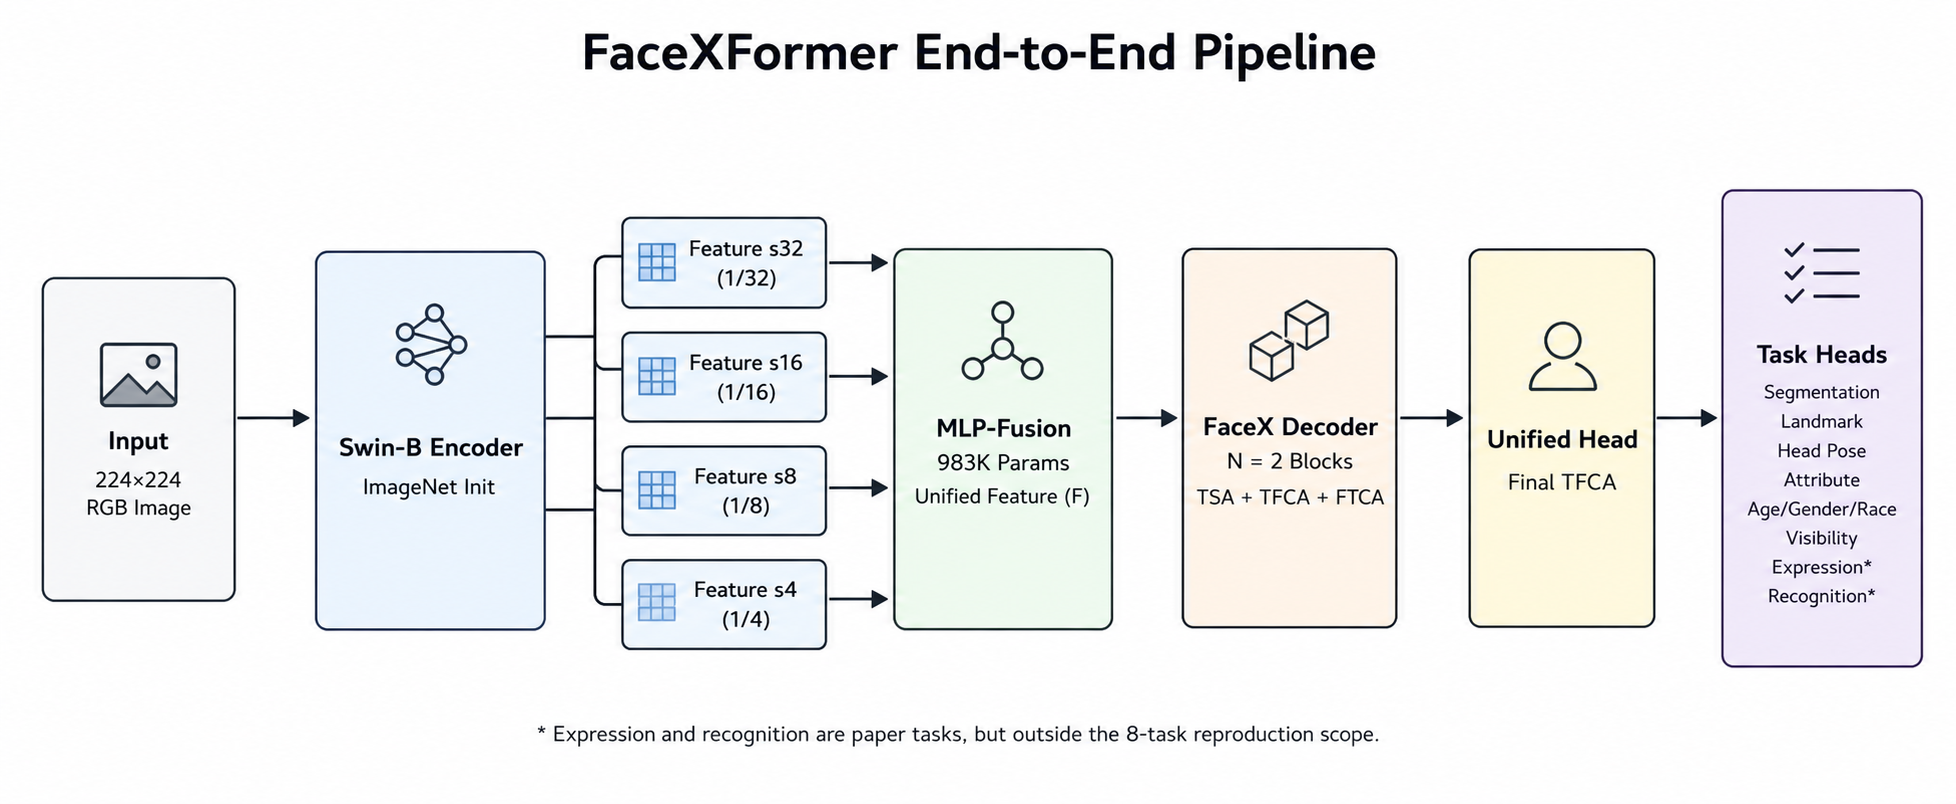
\includegraphics[width=0.98\textwidth]{assets/fig1_facexformer_pipeline.png}
\caption{FaceXFormer end-to-end pipeline. Input image is processed by a Swin-B encoder, fused via MLP-Fusion, then jointly decoded by the FaceX decoder operating on both face tokens and learnable task tokens.}
\end{figure}


\textbf{Divergence Note.} The high-level architecture is preserved for the eight reproduced tasks. The scope diverges from the paper because expression recognition and face recognition are absent from the implementation used here.


\subsection{Encoder: Swin-B Backbone}


\textbf{(Paper)} The encoder is an ImageNet-pretrained Swin-B transformer. It extracts four stages of hierarchical features, corresponding to progressively coarser spatial strides. The paper emphasizes that FaceXFormer does not use face-specific pretraining; the unified face representation is learned through multi-task co-training from an ImageNet-initialized backbone. This is an important design claim because it separates FaceXFormer from approaches that depend on large face-pretrained representation models.


\textbf{(Repo / Our impl.)} The code uses \path{torchvision.models.swin_b} as the backbone and projects the four encoder blocks into a shared decoder hidden size. The reproduced configuration uses a decoder embedding dimension of 256 and a decoder depth of 2.


\textbf{Divergence Note.} No major backbone divergence was identified. The relevant implementation question is not the backbone family, but the downstream token and head design.


\subsection{MLP-Fusion Module}


\textbf{(Paper)} The MLP-Fusion module follows the lightweight decoder-head design style used in SegFormer. Each of the four multi-scale feature maps is projected into a common target dimension, the projected maps are concatenated, and a final MLP fusion operation produces the unified face representation \(F\). The paper reports this module as lightweight, with approximately 983K parameters, and positions it as a key reason the model can use multi-scale information without the cost of a heavy pixel decoder.


\textbf{(Repo / Our impl.)} The reproduced model follows the same conceptual pattern: four Swin features are projected to a common 256-channel space, concatenated, and fused by a convolutional/MLP-style fusion block before being passed to the FaceX decoder.


\textbf{Divergence Note.} No major fusion-module divergence was found at the level needed for this report. The paper-level claim and the repository implementation agree on multi-scale projection, concatenation, and lightweight fusion.


\subsection{Task Tokens}


\textbf{(Paper)} FaceXFormer represents tasks using learnable task tokens. The paper explicitly states that segmentation uses one token per segmentation class, landmark prediction uses 68 tokens, and head pose uses 9 tokens corresponding to a 3x3 rotation matrix. It then states that one token is used for each of the other tasks. This matters because token count determines how much task-specific structure can be represented before the prediction head.


\textbf{(Repo / Our impl.)} The current code uses 18 task tokens total: 1 landmark token, 1 pose token, 1 attribute token, 1 visibility token, 1 age token, 1 gender token, 1 race token, and 11 segmentation mask tokens. The landmark token is passed through an MLP to output 136 coordinate values. The pose token is passed through an MLP to output 3 Euler-angle values. Attribute prediction uses one token and outputs 40 logits.


\emph{Table 3.1. Task Token Counts - Paper vs. Repo / Our Implementation}

\begingroup
\scriptsize
\setlength{\tabcolsep}{3pt}
\begin{longtable}{@{}>{\RaggedRight\arraybackslash}p{0.235\textwidth}>{\RaggedRight\arraybackslash}p{0.235\textwidth}>{\RaggedRight\arraybackslash}p{0.235\textwidth}>{\RaggedRight\arraybackslash}p{0.235\textwidth}@{}}
\toprule
Task & Paper Token Count & Repo / Our Implementation & Divergence \\
\midrule
\endfirsthead
\toprule
Task & Paper Token Count & Repo / Our Implementation & Divergence \\
\midrule
\endhead
Face Parsing / Segmentation & One per segmentation class; paper appendix mentions 19 CelebAMask-HQ classes & 11 mask tokens & \textbf{MED - class mapping/token count ambiguity} \\
Landmark Detection & 68 tokens, one per keypoint & 1 token $\rightarrow$ MLP $\rightarrow$ 136 coordinates & \textbf{HIGH - fundamentally different tokenization} \\
Head Pose Estimation & 9 tokens for a 3x3 rotation matrix & 1 token $\rightarrow$ MLP $\rightarrow$ 3 Euler angles & \textbf{HIGH - different representation and output geometry} \\
Attribute Prediction & 1 token; MLP outputs 40 attributes & 1 token $\rightarrow$ MLP $\rightarrow$ 40 logits & None confirmed \\
Age Estimation & 1 token & 1 token $\rightarrow$ MLP $\rightarrow$ 8 age bins & Minor output-bin implementation detail \\
Gender Classification & 1 token & 1 token $\rightarrow$ MLP $\rightarrow$ 2 logits & None \\
Race Classification & 1 token & 1 token $\rightarrow$ MLP $\rightarrow$ 5 logits & Minor class-taxonomy limitation \\
Face Visibility & 1 token & 1 token $\rightarrow$ MLP $\rightarrow$ 29 logits & None confirmed \\
Expression Recognition & 1 token & Not implemented & \textbf{HIGH - dropped task} \\
Face Recognition & 1 token & Not implemented & \textbf{HIGH - dropped task} \\
\bottomrule
\end{longtable}
\endgroup


\emph{Note. Task token counts as described in the paper compared with the released/reproduced implementation. The landmark and head-pose token divergences are the most consequential architecture-level mismatches.}

The landmark token discrepancy is especially important. A 68-token design can assign separate attention capacity to each landmark, allowing per-keypoint representations to interact with the face tokens and with each other. Collapsing all landmarks into a single token compresses the geometric signal before prediction. Even if the final MLP still emits 136 coordinate values, the attention mechanism no longer has one learned query per landmark. This likely weakens the landmark task as a source of spatially precise gradients for the shared face representation.


\textbf{Divergence Note.} The original outline stated that the paper used 40 attribute tokens. Cross-checking the paper text indicates otherwise: the paper says one token is used for other tasks after segmentation, landmarks, and head pose. Attribute prediction still outputs 40 binary labels, but those labels are produced from a single task token.


\subsection{FaceX Decoder}


\textbf{(Paper)} The FaceX decoder is the central architectural novelty. It uses \(N=2\) decoder blocks. Each block models interactions among task tokens and face tokens through three attention operations:


\begin{itemize}[leftmargin=*]
\item \textbf{Task Self-Attention (TSA):} task tokens attend to other task tokens, allowing task relationships to be modeled explicitly.
\item \textbf{Task-to-Face Cross-Attention (TFCA):} task tokens act as queries while face tokens act as keys and values, allowing each task to extract visual evidence from the fused face representation.
\item \textbf{Face-to-Task Cross-Attention (FTCA):} face tokens act as queries while task tokens act as keys and values, allowing the shared face representation to be refined by task-specific information.
\end{itemize}

The bidirectional aspect is the key difference from standard task-to-image decoders. In a standard cross-attention design, task tokens can read from the image representation, but the image representation itself is not updated by the task tokens. FaceXFormer adds the reverse direction through FTCA. The paper argues that this feedback loop improves the shared face representation, especially for tasks that depend on spatially detailed face tokens.


\textbf{(Repo / Our impl.)} The \path{TwoWayAttentionBlock} implementation matches the core paper structure: task self-attention, token-to-image cross-attention, an MLP block, and image-to-token cross-attention. The \path{TwoWayTransformer} stacks two such blocks and then applies a final token-to-image attention layer corresponding to the unified head. This is structurally consistent with the paper's two-block FaceX decoder description.


\begin{figure}[H]
\centering
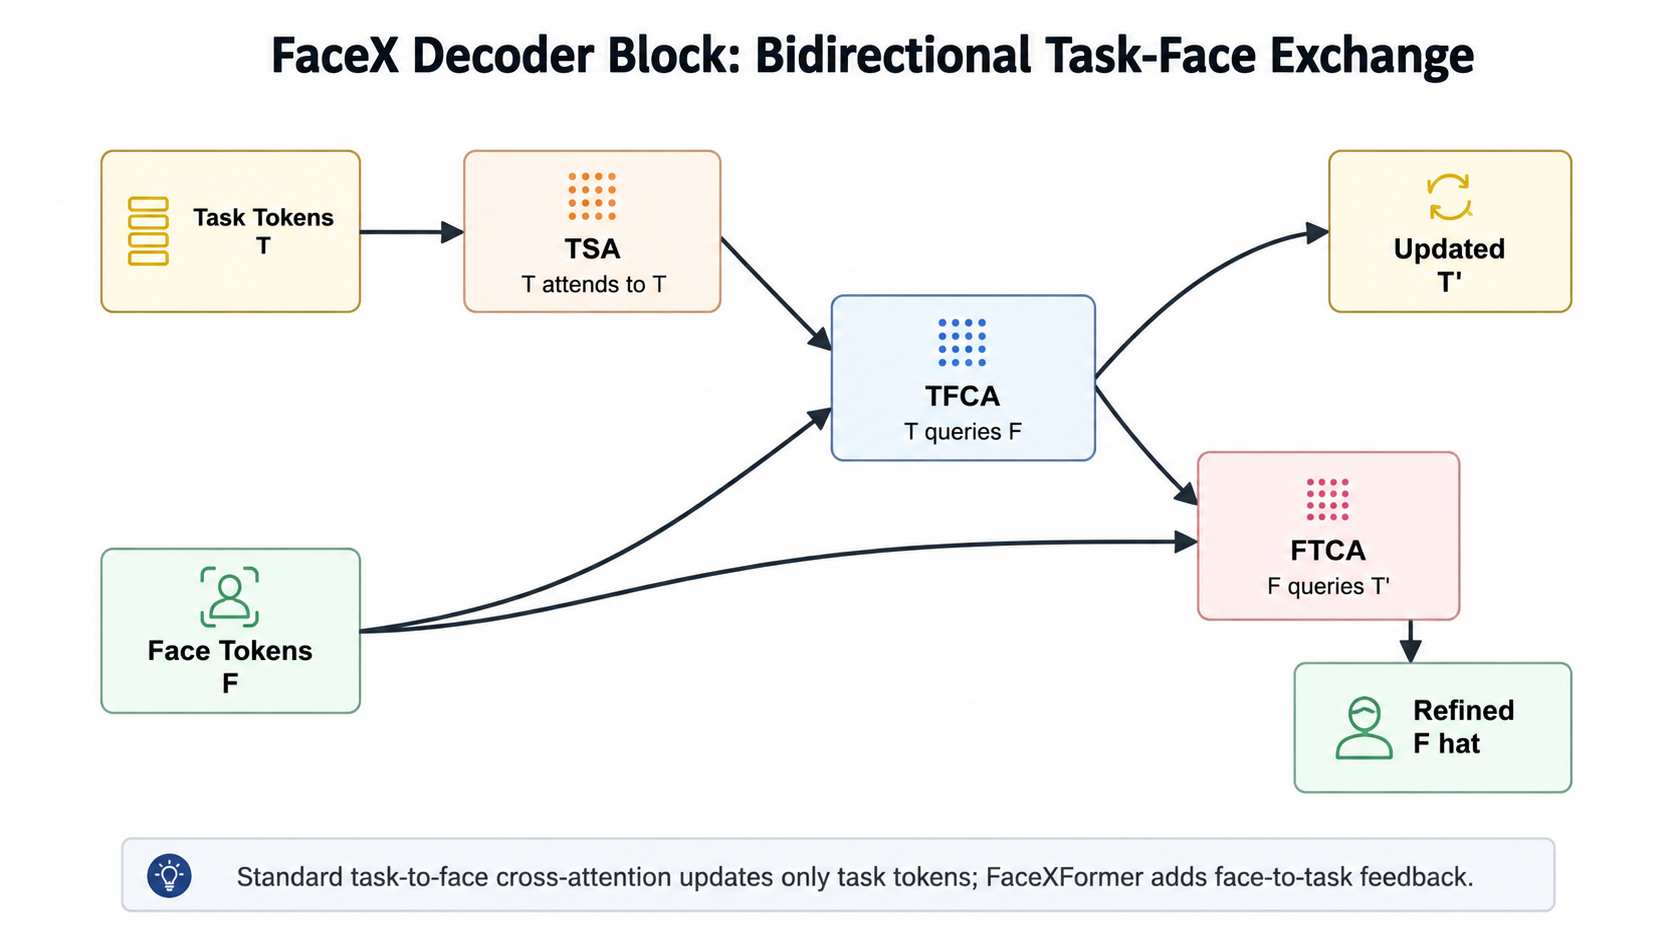
\includegraphics[width=0.86\textwidth]{assets/fig2_facex_decoder_block.png}
\caption{FaceX decoder block detail showing TSA, TFCA, and FTCA.}
\end{figure}


\textbf{Divergence Note.} No major decoder-operation divergence was found. The repository implements the bidirectional attention pattern that the paper claims. The larger discrepancies occur in token counts, task scope, and prediction heads.


\subsection{Unified Head and Task-Specific Prediction Heads}


\textbf{(Paper)} The unified head applies a final task-to-face cross-attention operation before task-specific prediction. The paper describes an hourglass network for landmark prediction, a regression MLP for head pose, PartialFC with ArcFace for face recognition, an upsampling and cross-product mechanism for segmentation, and classification or regression MLPs for the remaining tasks.


\textbf{(Repo / Our impl.)} The implementation uses a final token-to-image attention layer and then routes each token to lightweight heads. Segmentation uses 11 mask tokens, an upscaling module, and a hypernetwork-style cross-product with upscaled face features. Landmark prediction uses a single-token MLP outputting 136 coordinates. Head pose uses a single-token MLP outputting 3 Euler angles. Attributes, visibility, age, gender, and race use MLP heads. Expression recognition and face recognition heads are absent.


\emph{Table 3.2. Task Prediction Heads - Paper vs. Repo / Our Implementation}

\begingroup
\scriptsize
\setlength{\tabcolsep}{3pt}
\begin{longtable}{@{}>{\RaggedRight\arraybackslash}p{0.188\textwidth}>{\RaggedRight\arraybackslash}p{0.188\textwidth}>{\RaggedRight\arraybackslash}p{0.188\textwidth}>{\RaggedRight\arraybackslash}p{0.188\textwidth}>{\RaggedRight\arraybackslash}p{0.188\textwidth}@{}}
\toprule
Task & Paper Head & Repo / Our Implementation & Loss Function in Reproduction & Divergence \\
\midrule
\endfirsthead
\toprule
Task & Paper Head & Repo / Our Implementation & Loss Function in Reproduction & Divergence \\
\midrule
\endhead
Segmentation & Upsample + cross-product with segmentation tokens & Implemented with 11 mask tokens and upscaled face features & Dice + CE & Class mapping/token count ambiguity \\
Landmark & Hourglass network on 68 landmark tokens & MLP on 1 landmark token $\rightarrow$ 136 coordinates & STARLoss-style landmark loss & \textbf{HIGH} \\
Head Pose & Regression MLP from 9 rotation-matrix tokens & MLP on 1 pose token $\rightarrow$ 3 Euler angles & Geodesic loss via Euler-to-rotation conversion & \textbf{HIGH} \\
Attribute & Classification MLP & MLP on 1 token $\rightarrow$ 40 logits & BCE with logits & None confirmed \\
Age & Classification/regression MLP & MLP on 1 token $\rightarrow$ 8 age-bin logits & L1 + CE over age bins & Minor bin-boundary detail \\
Gender & Classification MLP & MLP on 1 token $\rightarrow$ 2 logits & CE & None \\
Race & Classification MLP & MLP on 1 token $\rightarrow$ 5 logits & CE & Class taxonomy differs from FairFace 7-class labels \\
Visibility & Classification MLP & MLP on 1 token $\rightarrow$ 29 logits & BCE with logits & None confirmed \\
Expression & Classification MLP & Not implemented & - & Dropped \\
Face Recognition & PartialFC + ArcFace & Not implemented & - & Dropped \\
\bottomrule
\end{longtable}
\endgroup


\emph{Note. Task-specific prediction heads and loss functions. The landmark and head-pose heads are the largest implementation divergences relative to the paper description.}

\textbf{Divergence Note.} The landmark head is the most consequential head-level mismatch: the paper describes an hourglass network operating after a 68-token landmark representation, whereas the reproduced implementation uses a single task token and a direct MLP. Head pose is also materially different because the paper describes a 3x3 rotation-matrix representation, while the implementation predicts 3 Euler angles. These choices change not only the task output parameterization but also the gradients that flow back through the FaceX decoder into the shared representation.


\section{Reproduction Methodology}


\subsection{Paper-vs-Code Gap Analysis}


The reproduction began with a structured audit of the FaceXFormer paper against the released repository. Each gap was categorized using four fields: \textbf{Paper Claim}, \textbf{Repo Reality}, \textbf{Our Resolution}, and \textbf{Impact}. Impact is used as a practical reproducibility label: \textbf{CRITICAL} means the reproduction cannot proceed without rebuilding the missing component; \textbf{HIGH} means the gap can materially change results; \textbf{MED} means the gap is measurable but bounded; \textbf{NONE} means no substantive divergence was found.


\emph{Table 4.1. Structured Paper-vs-Code Gap Analysis}

\begingroup
\scriptsize
\setlength{\tabcolsep}{3pt}
\begin{longtable}{@{}>{\RaggedRight\arraybackslash}p{0.157\textwidth}>{\RaggedRight\arraybackslash}p{0.157\textwidth}>{\RaggedRight\arraybackslash}p{0.157\textwidth}>{\RaggedRight\arraybackslash}p{0.157\textwidth}>{\RaggedRight\arraybackslash}p{0.157\textwidth}>{\RaggedRight\arraybackslash}p{0.157\textwidth}@{}}
\toprule
\# & Component & Paper Claim & Repo Reality & Our Resolution & Impact \\
\midrule
\endfirsthead
\toprule
\# & Component & Paper Claim & Repo Reality & Our Resolution & Impact \\
\midrule
\endhead
1 & Task scope & 10 tasks & 8 tasks; no expression or face recognition path & Reproduced 8 tasks; dropped expression and recognition & HIGH \\
2 & Task token count & Segmentation: one per class; landmarks: 68; head pose: 9; other tasks: 1 each & 18 total tokens: 11 mask + 1 token each for landmark, pose, attribute, visibility, age, gender, race & Followed repo tokenization for reproduced model; documented mismatch & HIGH \\
3 & Segmentation class mapping & One token per parsing class; paper appendix mentions 19 CelebAMask-HQ classes & Current implementation uses 11 mask tokens/classes & Used repo mapping; treated as class-mapping ambiguity & MED \\
4 & Landmark head & Hourglass network on 68 landmark tokens & Simple MLP on one landmark token & Used repo MLP and documented as architectural divergence & HIGH \\
5 & Head pose representation & 9 tokens representing a 3x3 rotation matrix & One pose token producing 3 Euler-angle values & Used repo representation; converted to rotation matrices for loss/eval where needed & HIGH \\
6 & Loss coefficients & Joint weighted objective, but lambda values not published & No public loss implementation in released inference code & Reported reproduction used lambda\_i = 1.0 following author email confirmation & HIGH \\
7 & Training loop & Implied by paper results & Not released & Rebuilt PyTorch DDP training loop with checkpointing and evaluation & CRITICAL \\
8 & Dataset loaders & Implied for all paper datasets & Not released & Built task-specific dataset adapters for the 8 reproduced tasks & CRITICAL \\
9 & Multi-task sampler & Upsampling-based balancing described only at high level & Not released & Implemented upsampling and balanced per-batch task sampling & HIGH \\
10 & Epoch schedule & 12 epochs plus unspecified extra epochs for some tasks & Extra-task schedule absent & Trained 12 epochs for all reproduced tasks & MED \\
11 & Augmentation & Appendix F describes task-specific augmentations & No released training augmentations & Implemented task-specific augmentation pipelines from appendix/code reconstruction & MED \\
12 & Expression recognition & Included in paper results & Absent from codebase & Dropped; RAF-DB/AffectNet not included in final scope & HIGH \\
13 & Face recognition & PartialFC + ArcFace on MS1MV3 & Absent from codebase & Dropped; MS1MV3 and PartialFC training were compute/data prohibitive & HIGH \\
\bottomrule
\end{longtable}
\endgroup


\emph{Note. Complete paper-vs-code gap analysis. Impact ratings describe how strongly each gap affects independent reproduction.}

This audit shows that FaceXFormer is a weights-only release for training reproducibility purposes. The checkpoint and inference code are valuable for baseline verification, but they do not define the training process that produced the reported multi-task model. The most critical omissions are the missing training loop, missing dataset loaders, missing sampler, and unpublished loss coefficients. The architecture also contains consequential mismatches between the paper description and the released/reproduced implementation, especially for landmark detection and head pose estimation.


\begin{figure}[H]
\centering
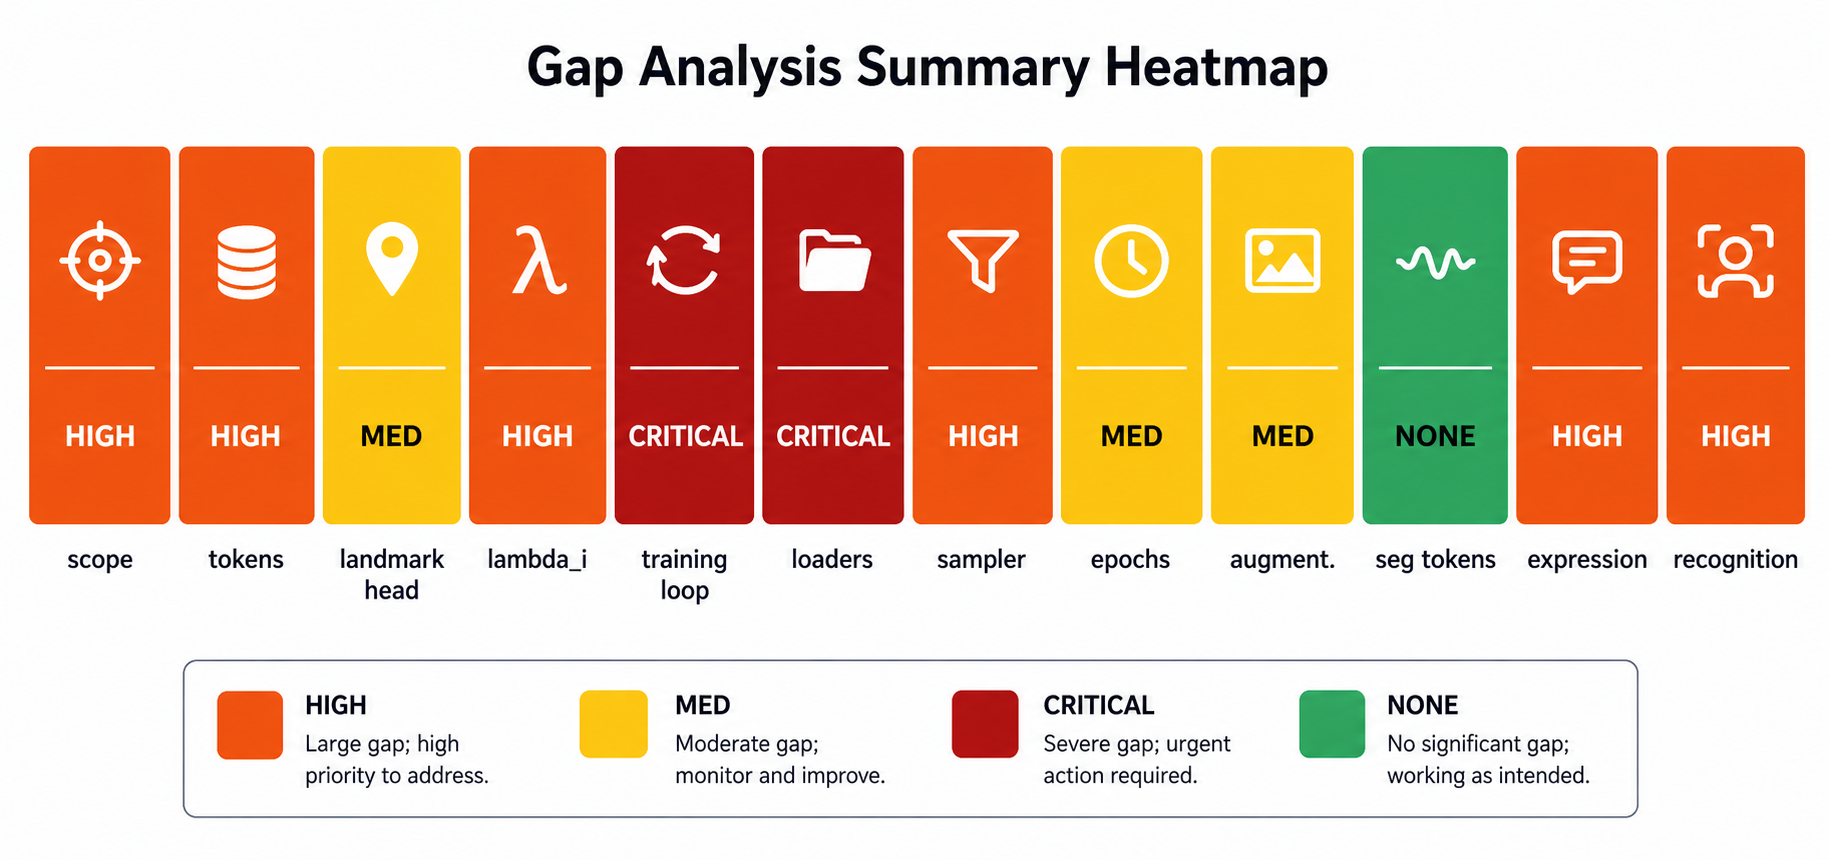
\includegraphics[width=0.98\textwidth]{assets/fig8_gap_analysis_heatmap.png}
\caption{Gap analysis summary heatmap.}
\end{figure}


\subsection{Dataset Preparation}


The reproduced pipeline covers eight tasks and uses task-specific train/evaluation adapters. Evaluation includes the primary paper-comparable datasets plus diagnostic cross-dataset rows used to understand generalization and protocol mismatch.


\emph{Table 4.2. Datasets, Splits, and Sample Counts}

\begingroup
\scriptsize
\setlength{\tabcolsep}{3pt}
\begin{longtable}{@{}>{\RaggedRight\arraybackslash}p{0.157\textwidth}>{\RaggedRight\arraybackslash}p{0.157\textwidth}>{\RaggedRight\arraybackslash}p{0.157\textwidth}>{\RaggedRight\arraybackslash}p{0.157\textwidth}>{\RaggedRight\arraybackslash}p{0.157\textwidth}>{\RaggedRight\arraybackslash}p{0.157\textwidth}@{}}
\toprule
Task & Dataset & Train Split & Evaluation Split & Eval Samples & Preprocessing \\
\midrule
\endfirsthead
\toprule
Task & Dataset & Train Split & Evaluation Split & Eval Samples & Preprocessing \\
\midrule
\endhead
Segmentation & CelebAMask-HQ & 24,000 to 28,000, depending on split convention & Test & 2,000 & Resize to 224x224; repo maps masks to 11 classes \\
Landmark & 300W & 3,148 & Full test set & 689 & 5-point affine/ArcFace-style alignment; 68 keypoints \\
Head Pose & 300W-LP train, BIWI eval & 122,450 for 300W-LP & BIWI & 15,678 & Loose crop / resized crop; preserve pose labels \\
Attribute & CelebA & 162,770 & CelebA test & 19,962 & 40 binary labels; aligned face crops \\
Attribute & LFWA & Not used for training & LFWA & 13,143 & Cross-dataset diagnostic only \\
Age & UTKFace & Train split & UTKFace eval split & 3,556 & Age parsed from filename; mapped to age bins as needed \\
Age & FairFace & Train split & FairFace eval split & 21,908 & Age-group labels; multi-ethnic distribution \\
Gender & UTKFace & Shared with age/race & UTKFace eval split & 3,556 & Binary label \\
Gender & FairFace & Shared with age/race & FairFace eval split & 21,908 & Binary label \\
Race & UTKFace & Shared with age/gender & UTKFace eval split & 3,556 & 5-class label \\
Race & FairFace & Shared with age/gender & FairFace eval split & 21,908 & 7-class source labels mapped into repo-compatible taxonomy where needed \\
Visibility & COFW & 1,345 & Test & 507 & 29 per-landmark visibility/occlusion labels \\
\bottomrule
\end{longtable}
\endgroup


\emph{Note. Datasets used for the eight-task reproduction and evaluation. Counts reflect the current fixed evaluation manifest where available.}

\textbf{Sample count reconciliation.} The report outline and presentation use 127,735 total evaluation samples across 12 dataset-task combinations. The fresh fixed manifest in \path{results/baseline_current_8task_fresh_fixed/} reports 129,060 samples across 14 result rows because it includes 300W common/challenging subset rows in addition to the 300W full row. It also evaluates 300W full as 689 images, matching the paper appendix, whereas the outline table lists a 53-sample landmark row. In this report, we use dataset-specific counts from the current manifest when discussing concrete evaluation runs, and we reserve the 127,735 figure for the original scoped presentation total.


Landmark preprocessing required an engineering choice not fully specified in the paper. The reproduction derives five anchor points from the 68 landmark annotations and applies an ArcFace-style affine alignment before resizing to the target resolution. During training, geometric transforms are applied jointly to the image and landmarks so the labels remain consistent. LFWA is treated as a diagnostic cross-dataset attribute evaluation; it is not a paper target row and should not be interpreted as a reproduction failure.


\subsection{Augmentation Pipeline}


Task-specific augmentations were implemented in \path{datasets.py} and applied only during training. Evaluation uses clean resized/aligned inputs with ImageNet normalization. The paper appendix describes augmentation categories, but not every probability and implementation detail is fully specified. Where the paper was ambiguous, the reproduction used the closest task-appropriate implementation and documented the choice.


\emph{Table 4.3. Augmentation Operations and Per-Task Application}

\begingroup
\scriptsize
\setlength{\tabcolsep}{3pt}
\begin{longtable}{@{}>{\RaggedRight\arraybackslash}p{0.117\textwidth}>{\RaggedRight\arraybackslash}p{0.117\textwidth}>{\RaggedRight\arraybackslash}p{0.117\textwidth}>{\RaggedRight\arraybackslash}p{0.117\textwidth}>{\RaggedRight\arraybackslash}p{0.117\textwidth}>{\RaggedRight\arraybackslash}p{0.117\textwidth}>{\RaggedRight\arraybackslash}p{0.117\textwidth}>{\RaggedRight\arraybackslash}p{0.117\textwidth}@{}}
\toprule
Augmentation & Parameters & Segmentation & Landmark & Head Pose & Attribute & Age/Gender/Race & Visibility \\
\midrule
\endfirsthead
\toprule
Augmentation & Parameters & Segmentation & Landmark & Head Pose & Attribute & Age/Gender/Race & Visibility \\
\midrule
\endhead
Resize / normalization & 224x224; ImageNet mean/std & Yes & Yes & Yes & Yes & Yes & Yes \\
ArcFace-style alignment & 5-point template & No & Yes & No & No & No & No \\
Random rotation & +/-18 deg & No & Yes & No & Yes & Yes & No \\
Random scaling & 0.9 to 1.1 & No & Yes & No & Yes & Yes & No \\
Random translation / crop & 1 to 5 percent or resized crop & No & Yes & Crop proxy & Yes & Yes & No \\
Horizontal flip & p = 0.5 with label remapping when needed & No & Yes & No & Yes & Yes & Yes \\
Grayscale & p = 0.1 to 0.2 & No & Yes & Yes & Yes & Yes & Yes \\
Gaussian blur & radius 0.5 to 2.0 px & No & Yes & Yes & Yes & Yes & Yes \\
Random occlusion & random patch & No & Yes & No & No & No & No \\
Gamma adjustment & gamma in [0.7, 1.3] & No & Yes & Yes & Yes & Yes & Yes \\
\bottomrule
\end{longtable}
\endgroup


\emph{Note. Task-specific augmentation operations in the reproduced training pipeline. Head pose and visibility avoid geometric transforms that would invalidate labels unless labels can be transformed consistently.}

This differs slightly from the high-level outline because the actual implementation is more conservative for segmentation, head pose, and visibility. Segmentation uses clean resizing and normalization in the current dataset adapter. Head pose uses a random resized crop proxy plus photometric perturbations rather than arbitrary in-plane rotation, because rotating the image without updating the pose label would corrupt the supervision. Visibility supports horizontal flip by reordering the 29 visibility labels using a symmetric landmark mapping.


\subsection{Loss Functions}


The paper defines a weighted joint objective over tasks:


\[
\mathcal{L} =
\lambda_{\text{seg}} \mathcal{L}_{\text{seg}}
+ \lambda_{\text{lnd}} \mathcal{L}_{\text{lnd}}
+ \lambda_{\text{hpe}} \mathcal{L}_{\text{hpe}}
+ \lambda_{\text{attr}} \mathcal{L}_{\text{attr}}
+ \lambda_{\text{age}} \mathcal{L}_{\text{age}}
+ \lambda_{\text{g/r}} \mathcal{L}_{\text{g/r}}
+ \lambda_{\text{vis}} \mathcal{L}_{\text{vis}} .
\]

The full paper objective also includes expression and face recognition terms, but those tasks are outside the eight-task reproduction scope. For the reported reproduction run, all task weights were set to \path{lambda_i = 1.0} following author email confirmation. The paper does not publish these values. The current repository contains later exploratory non-uniform \path{LOSS_WEIGHTS}; those tuned values are not treated as the paper-faithful reproduction setting.


\textbf{Segmentation loss.} \path{L_seg} is the mean of Dice loss and pixelwise cross-entropy over the reproduced segmentation classes. Dice loss addresses class imbalance in small facial regions, while cross-entropy provides dense per-pixel gradients.


\textbf{Landmark loss.} \path{L_lnd} is a STARLoss-style landmark loss applied to the 68-keypoint output of the reproduced MLP head. This is already downstream of an architectural divergence: the paper specifies an hourglass head operating from a 68-token landmark representation, while the reproduced model uses a single landmark token and emits 136 coordinate values.


\textbf{Head pose loss.} \path{L_hpe} is geodesic loss on SO(3). The implementation predicts Euler angles, converts prediction and target into rotation matrices, and computes the angular distance between rotations. This is geometrically more appropriate than direct Euclidean distance, but it differs from the paper's stated 9-token rotation-matrix output.


\textbf{Attribute loss.} \path{L_attr} is binary cross-entropy with logits over 40 CelebA attributes. Each attribute is treated as an independent binary label and the loss is averaged over labels and samples.


\textbf{Age loss.} \path{L_age} combines cross-entropy over age bins with an L1-style age expectation term. The reproduced implementation uses eight age groups with representative bin centers. This differs from a fully continuous age regression objective and should be treated as an implementation decision where the paper is underspecified.


\textbf{Gender and race loss.} \path{L_g/r} is standard cross-entropy. Gender uses two classes. Race uses the repo-compatible class taxonomy, with UTKFace and FairFace requiring careful handling because their race labels do not use identical class sets.


\textbf{Visibility loss.} \path{L_vis} is binary cross-entropy with logits over 29 per-landmark visibility values. Invalid or missing visibility entries are filtered before averaging when necessary.


\subsection{Task-Balanced Multi-Task Sampler}


The reproduction implements an upsampling-based multi-task sampler. For each task, smaller datasets are repeated and shuffled until they match the effective size of the largest task pool. A custom balanced batch sampler then draws a fixed or near-fixed number of samples from each active task in every batch. When the batch size is not divisible by the number of active tasks, the extra sample slots are randomly assigned across tasks per batch to prevent systematic bias. This implements the paper's high-level upsampling description, but the paper does not specify whether the original authors used pure repetition, weighted sampling, shuffled repetition, or another balancing rule.


\subsection{Training Configuration}


\emph{Table 4.4. Full Training Configuration}

\begingroup
\scriptsize
\setlength{\tabcolsep}{3pt}
\begin{longtable}{@{}>{\RaggedRight\arraybackslash}p{0.380\textwidth}>{\RaggedRight\arraybackslash}p{0.380\textwidth}@{}}
\toprule
Parameter & Value \\
\midrule
\endfirsthead
\toprule
Parameter & Value \\
\midrule
\endhead
Hardware & 8 x NVIDIA A100 GPUs on Purdue institutional cluster \\
Framework & PyTorch with DistributedDataParallel \\
Distributed backend & NCCL \\
Precision & FP16 mixed precision for cluster-scale runs \\
Batch size & 48 per GPU, 384 effective \\
Optimizer & AdamW \\
Initial learning rate & 1e-4 \\
LR decay & multiply by 0.1 at epochs 6 and 10 \\
Weight decay & 1e-5 \\
Total epochs & 12 \\
Additional epochs & Not applied; paper does not identify which tasks receive extra epochs \\
Backbone initialization & ImageNet-pretrained Swin-B \\
Input resolution & 224x224 \\
Loss coefficients & lambda\_i = 1.0 for reported paper-faithful reproduction \\
Checkpointing & Per-epoch checkpointing and resume support \\
Gradient stabilization & Gradient clipping in training loop \\
\bottomrule
\end{longtable}
\endgroup


\emph{Note. Training hyperparameters used for the reported reproduction. Later exploratory config edits are not treated as the paper-faithful setting.}

\subsection{Staged Training Strategy}


The eight-task training run was staged to reduce the risk of debugging all tasks simultaneously. Stage 1 trained the geometric core: segmentation, landmark detection, and head pose estimation. This validated the sampler, dense prediction path, coordinate regression path, and pose loss. Stage 2 added attribute prediction, age estimation, and gender classification, expanding the system to multi-label and categorical classification tasks with different loss scales. Stage 3 added race and visibility, producing the full eight-task reproduction. Each stage initialized from the checkpoint produced by the previous stage.


\begin{figure}[H]
\centering
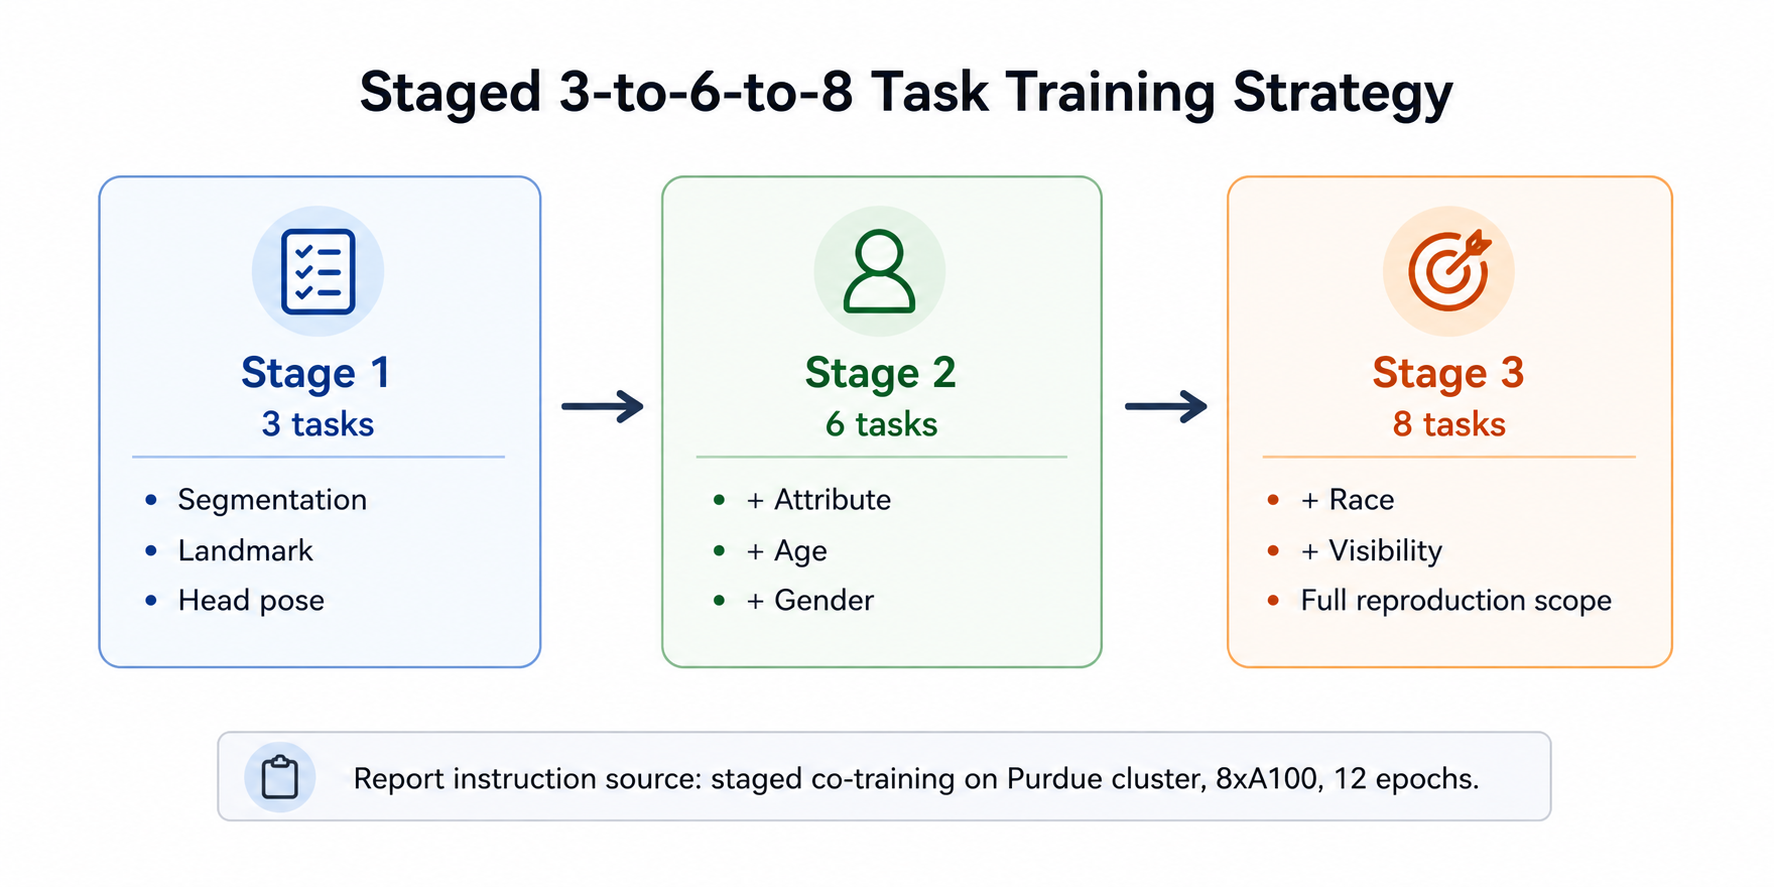
\includegraphics[width=0.88\textwidth]{assets/fig3_staged_training_timeline.png}
\caption{Staged 3-to-6-to-8 task training strategy.}
\end{figure}


\subsection{Metric Normalization Framework}


A major reproducibility problem was that raw script outputs were not always in the same unit as paper-reported metrics. The reproduction therefore records both raw and normalized values and uses explicit normalization rules from the baseline manifest.


\emph{Table 4.5. Metric Normalization Rules}

\begingroup
\scriptsize
\setlength{\tabcolsep}{3pt}
\begin{longtable}{@{}>{\RaggedRight\arraybackslash}p{0.188\textwidth}>{\RaggedRight\arraybackslash}p{0.188\textwidth}>{\RaggedRight\arraybackslash}p{0.188\textwidth}>{\RaggedRight\arraybackslash}p{0.188\textwidth}>{\RaggedRight\arraybackslash}p{0.188\textwidth}@{}}
\toprule
Task & Raw Script Output & Paper Unit & Normalization & Example \\
\midrule
\endfirsthead
\toprule
Task & Raw Script Output & Paper Unit & Normalization & Example \\
\midrule
\endhead
Segmentation & F1 fraction & F1 percent & multiply by 100 & 0.9177 $\rightarrow$ 91.77\% \\
Landmark & NME percent & NME percent & no conversion & 6.75 $\rightarrow$ 6.75\% \\
Head Pose & MAE in degrees in current fixed manifest & MAE degrees & no conversion in fixed manifest & 20.65 $\rightarrow$ 20.65 deg \\
Attribute & Accuracy fraction & Accuracy percent & multiply by 100 & 0.9172 $\rightarrow$ 91.72\% \\
Age & MAE in years & MAE years & no conversion & 1.17 $\rightarrow$ 1.17 years \\
Gender & Accuracy fraction & Accuracy percent & multiply by 100 & 0.9918 $\rightarrow$ 99.18\% \\
Race & Accuracy fraction & Accuracy percent & multiply by 100 & 0.9803 $\rightarrow$ 98.03\% \\
Visibility & Recall fraction & Recall percent & multiply by 100 & 0.8713 $\rightarrow$ 87.13\% \\
\bottomrule
\end{longtable}
\endgroup


\emph{Note. Normalization rules used to convert raw evaluation outputs to report-ready units. Source: \path{results/baseline_current_8task_fresh_fixed/baseline_current_8task_manifest.json}.}

The scientific point is simple: without a normalization layer, evaluation numbers can look catastrophically wrong for reasons unrelated to model quality. A raw fraction such as 0.9177 is not a 0.92\% segmentation result; it is 91.77\% after conversion. Similarly, older smoke and metric-check runs mixed raw radians, degrees, fractions, and percentages in ways that made direct paper comparison unsafe. The fixed manifest makes the unit convention explicit through its \path{normalization_rules} field. That kind of metric documentation is infrastructure, not cosmetic reporting.


\section{Baseline Verification}


This section evaluates the released FaceXFormer checkpoint in inference-only mode. The purpose is not to train a model, but to verify whether the public checkpoint is loadable and whether its predictions can reproduce the paper's reported metrics under the eight-task evaluation pipeline reconstructed in this project.


\subsection{Experimental Setup}


We loaded the released checkpoint at \path{checkpoints/ckpts/model.pt} and ran task-specific evaluation on the corresponding dataset splits. The checkpoint is 1,104,869,851 bytes and has SHA256 hash \texttt{327A755849BA64D3\allowbreak{}36FB96589FF87B27\allowbreak{}E84A12BE1ECF8BCF\allowbreak{}AA503D66F803286D}. The fixed baseline manifest reports \path{checkpoint_loaded: true}, confirming that the checkpoint is functional in the reproduced code path. The run was generated under \path{results/baseline_current_8task_fresh_fixed/} with dataset, batch size 64, seed 0, and no sample cap. The run scope is the current eight-task implementation, not the full ten-task paper system.


For each task, the evaluator recorded raw metrics, normalized metrics, normalized units, paper targets where available, and paper-relative gaps. The fixed manifest contains 14 result rows and 129,060 evaluated samples because it includes diagnostic 300W common/challenging subset rows in addition to 300W full.


\subsection{Results}


\emph{Table 5.1. Baseline Inference Results - Released Checkpoint vs. Paper Targets}

\begingroup
\scriptsize
\setlength{\tabcolsep}{3pt}
\begin{longtable}{@{}>{\RaggedRight\arraybackslash}p{0.104\textwidth}>{\RaggedRight\arraybackslash}p{0.104\textwidth}>{\RaggedRight\arraybackslash}p{0.104\textwidth}>{\RaggedRight\arraybackslash}p{0.104\textwidth}>{\RaggedRight\arraybackslash}p{0.104\textwidth}>{\RaggedRight\arraybackslash}p{0.104\textwidth}>{\RaggedRight\arraybackslash}p{0.104\textwidth}>{\RaggedRight\arraybackslash}p{0.104\textwidth}>{\RaggedRight\arraybackslash}p{0.104\textwidth}@{}}
\toprule
Task & Dataset & Samples & Metric & Paper Target & Raw Value & Normalized Value & Gap & Status \\
\midrule
\endfirsthead
\toprule
Task & Dataset & Samples & Metric & Paper Target & Raw Value & Normalized Value & Gap & Status \\
\midrule
\endhead
Segmentation & CelebAMask-HQ & 2,000 & F1 (\%) & 92.01 & 0.9177 & 91.77 & -0.24 pp & MATCH \\
Landmark & 300W full & 689 & NME (\%) & 4.67 & 6.7528 & 6.75 & +2.08 & CLOSE GAP \\
Landmark & 300W common & 554 & NME (\%) & - & 5.5955 & 5.60 & - & Diagnostic \\
Landmark & 300W challenging & 135 & NME (\%) & - & 11.5021 & 11.50 & - & Diagnostic \\
Head Pose & BIWI & 15,678 & MAE (deg) & 3.52 & 20.6497 & 20.65 & +17.13 deg & LARGE GAP \\
Attribute & CelebA & 19,962 & Acc (\%) & 91.83 & 0.9172 & 91.72 & -0.11 pp & MATCH \\
Attribute & LFWA & 13,143 & Acc (\%) & - & 0.6106 & 61.06 & - & Cross-dataset \\
Age & UTKFace & 3,556 & MAE (years) & 4.17 & 1.1714 & 1.17 & -3.00 years & SUSPECT \\
Age & FairFace & 21,908 & MAE (years) & - & 6.2990 & 6.30 & - & No target \\
Gender & UTKFace & 3,556 & Acc (\%) & - & 0.9918 & 99.18 & - & No target \\
Gender & FairFace & 21,908 & Acc (\%) & - & 0.9311 & 93.11 & - & Diagnostic \\
Race & UTKFace & 3,556 & Acc (\%) & - & 0.9803 & 98.03 & - & No target \\
Race & FairFace & 21,908 & Acc (\%) & - & 0.6459 & 64.59 & - & Diagnostic \\
Visibility & COFW & 507 & Recall@P80 (\%) & 72.56 & 0.8713 & 87.13 & +14.57 pp & ABOVE PAPER \\
\bottomrule
\end{longtable}
\endgroup


\emph{Note. Baseline inference results for the released checkpoint. Source: \path{results/baseline_current_8task_fresh_fixed/gap_analysis_baseline_current_8task.json}. MATCH indicates within 1 percentage point of the paper target when the metric is a percentage. Diagnostic rows do not have direct paper targets under this reproduction protocol.}

\begin{figure}[H]
\centering
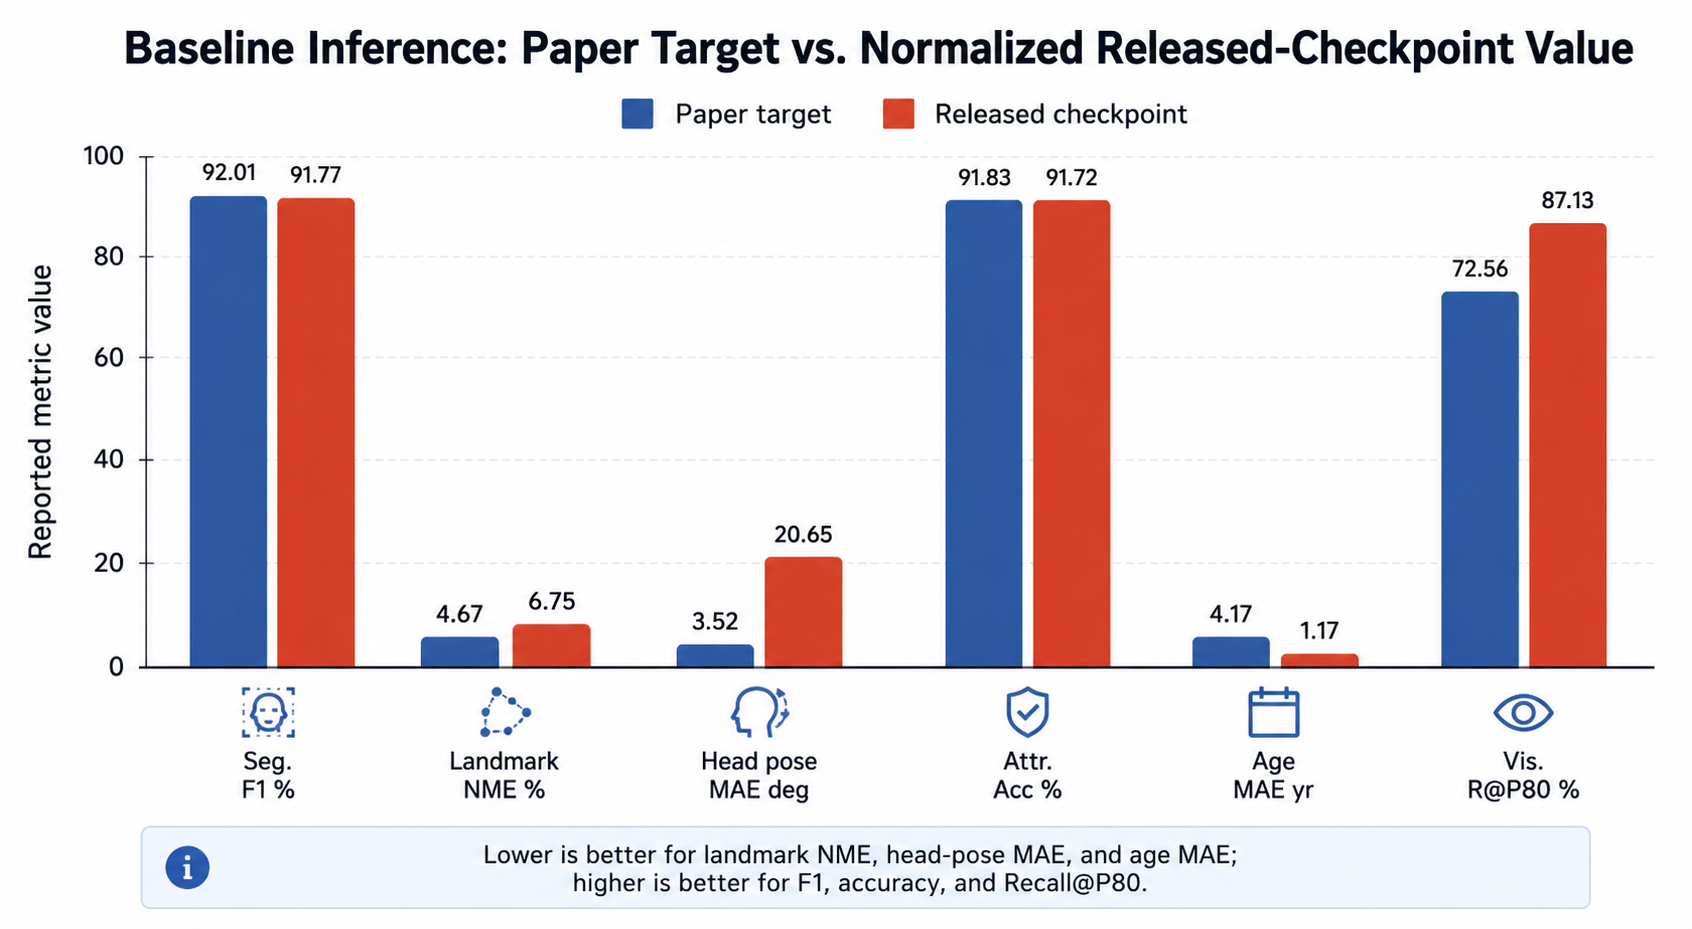
\includegraphics[width=0.98\textwidth]{assets/fig4_baseline_inference_bars.png}
\caption{Baseline inference bar chart comparing paper targets and normalized released-checkpoint values for paper-target rows.}
\end{figure}


\subsection{Analysis}


The strongest validation comes from segmentation and CelebA attributes. Segmentation reaches 91.77\% F1 against the paper target of 92.01\%, a gap of only -0.24 percentage points. Attribute prediction reaches 91.72\% accuracy against the paper target of 91.83\%, a gap of -0.11 percentage points. These two near-matches show that the released checkpoint is meaningful, the core inference path is functional, and the reconstructed normalization framework is sufficient for at least two major paper-target tasks.


Landmark detection is plausible but behind the paper. On 300W full, the released checkpoint obtains 6.75 NME compared with the paper's 4.67 target. The common/challenging subset split is also informative: 5.60 NME on common and 11.50 NME on challenging. This pattern is qualitatively reasonable because the challenging subset contains harder poses, occlusions, and expression variation. The remaining gap may reflect the landmark architecture discrepancy documented in Section 3, protocol differences, or residual preprocessing mismatch.


Head pose remains the largest unresolved baseline mismatch. The fixed manifest reports 20.65 degrees MAE on BIWI compared with the paper target of 3.52 degrees. Earlier intermediate runs mixed radians and degrees, but the fresh fixed manifest records head pose as degrees already; therefore this is not simply a display-unit error in the final baseline table. It should be treated as a real unresolved protocol or implementation gap until the pose preprocessing, axis convention, crop generation, and rotation conversion are verified against the original evaluation protocol.


Age and visibility should be interpreted carefully. UTKFace age MAE is 1.17 years, which is substantially better than the paper target of 4.17 years and is therefore suspicious rather than a clean success. Possible explanations include a split mismatch, label-bin conversion issue, leakage, or a metric computation difference. Visibility reaches 87.13\% Recall@P80 on COFW compared with the paper target of 72.56\%, also above paper. This may reflect a corrected recall computation or a protocol difference in how precision thresholds and visibility labels are defined.


The remaining rows are useful diagnostics rather than direct paper comparisons. LFWA attribute accuracy drops to 61.06\%, showing a large cross-dataset generalization gap relative to CelebA. FairFace gender reaches 93.11\%, while FairFace race reaches 64.59\% under a repo-compatible mapping; the latter is especially sensitive to class-taxonomy mismatch because FairFace has seven race categories while the current model head uses five. Overall, the baseline run largely validates the released checkpoint for segmentation and attributes, but it also exposes unresolved evaluation-protocol risks for head pose, age, visibility, and cross-dataset demographic tasks.


\section{8-Task Training Results}


\textbf{Preliminary status.} A bug has been identified in the training evaluation path affecting the landmark, head pose, and age rows. Results for these three tasks are under active investigation and should not be used as paper-comparable final results. Segmentation, attribute, gender, race, and visibility are treated as reportable preliminary rows, with gender/race/visibility still marked where their values suggest metric or class-distribution issues.


\subsection{Training Procedure}


The full training configuration is given in Table 4.4. Staged co-training completed all three phases: a 3-task geometric stage, a 6-task mixed regression/classification stage, and the final 8-task stage. Checkpoints were saved throughout training, and the preliminary evaluation reported here uses the epoch-12 checkpoint from the full 8-task run on the Purdue cluster using 8 x A100 GPUs. Because raw bug-fixed training logs were not available in the current repository package, the values in this section are explicitly treated as provenance-tagged preliminary results transcribed from the final presentation/report instruction source.


\subsection{Results}


\emph{Table 6.1. Preliminary 8-Task Training Results vs. Paper Targets}

\begingroup
\scriptsize
\setlength{\tabcolsep}{3pt}
\begin{longtable}{@{}>{\RaggedRight\arraybackslash}p{0.117\textwidth}>{\RaggedRight\arraybackslash}p{0.117\textwidth}>{\RaggedRight\arraybackslash}p{0.117\textwidth}>{\RaggedRight\arraybackslash}p{0.117\textwidth}>{\RaggedRight\arraybackslash}p{0.117\textwidth}>{\RaggedRight\arraybackslash}p{0.117\textwidth}>{\RaggedRight\arraybackslash}p{0.117\textwidth}>{\RaggedRight\arraybackslash}p{0.117\textwidth}@{}}
\toprule
Task & Dataset & Metric & Paper Target & Our Result & Gap & Verdict & Bug? \\
\midrule
\endfirsthead
\toprule
Task & Dataset & Metric & Paper Target & Our Result & Gap & Verdict & Bug? \\
\midrule
\endhead
Segmentation & CelebAMask-HQ & F1 (\%) & 92.01 & 85.91 & -6.10 pp & Close but below paper & No \\
Landmark & 300W & NME (\%) & 4.67 full / 3.05 common & 0.0117 & - & BUG - not comparable & Yes \\
Head Pose & BIWI & MAE (deg) & 3.52 & 0.379 & - & BUG - not comparable & Yes \\
Attribute & CelebA & Acc (\%) & 91.83 & 91.27 & -0.56 pp & Match & No \\
Attribute & LFWA & Acc (\%) & - & 59.87 & - & Cross-dataset & No \\
Age & UTKFace & MAE (years) & 4.17 & 35.27 & +31.10 years & BUG - not comparable & Yes \\
Age & FairFace & MAE (years) & - & 31.50 & - & BUG - not comparable & Yes \\
Gender & UTKFace & Acc (\%) & - & 85.04 & - & Plausible diagnostic & No \\
Gender & FairFace & Acc (\%) & 95.22 & 100.00 & +4.78 pp & Suspect & No \\
Race & UTKFace & Acc (\%) & - & 73.26 & - & Diagnostic & No \\
Race & FairFace & Acc (\%) & - & 99.96 & - & Suspect & No \\
Visibility & COFW & Recall@P80 (\%) & 72.56 & 99.25 & +26.69 pp & Suspect & No \\
\bottomrule
\end{longtable}
\endgroup


\emph{Note. Preliminary 8-task training results. Landmark, head pose, and age rows are affected by an identified training/evaluation bug and must not be compared directly to paper targets. Suspect rows greatly exceed paper targets or expected behavior and require metric/protocol verification.}

\begin{figure}[H]
\centering
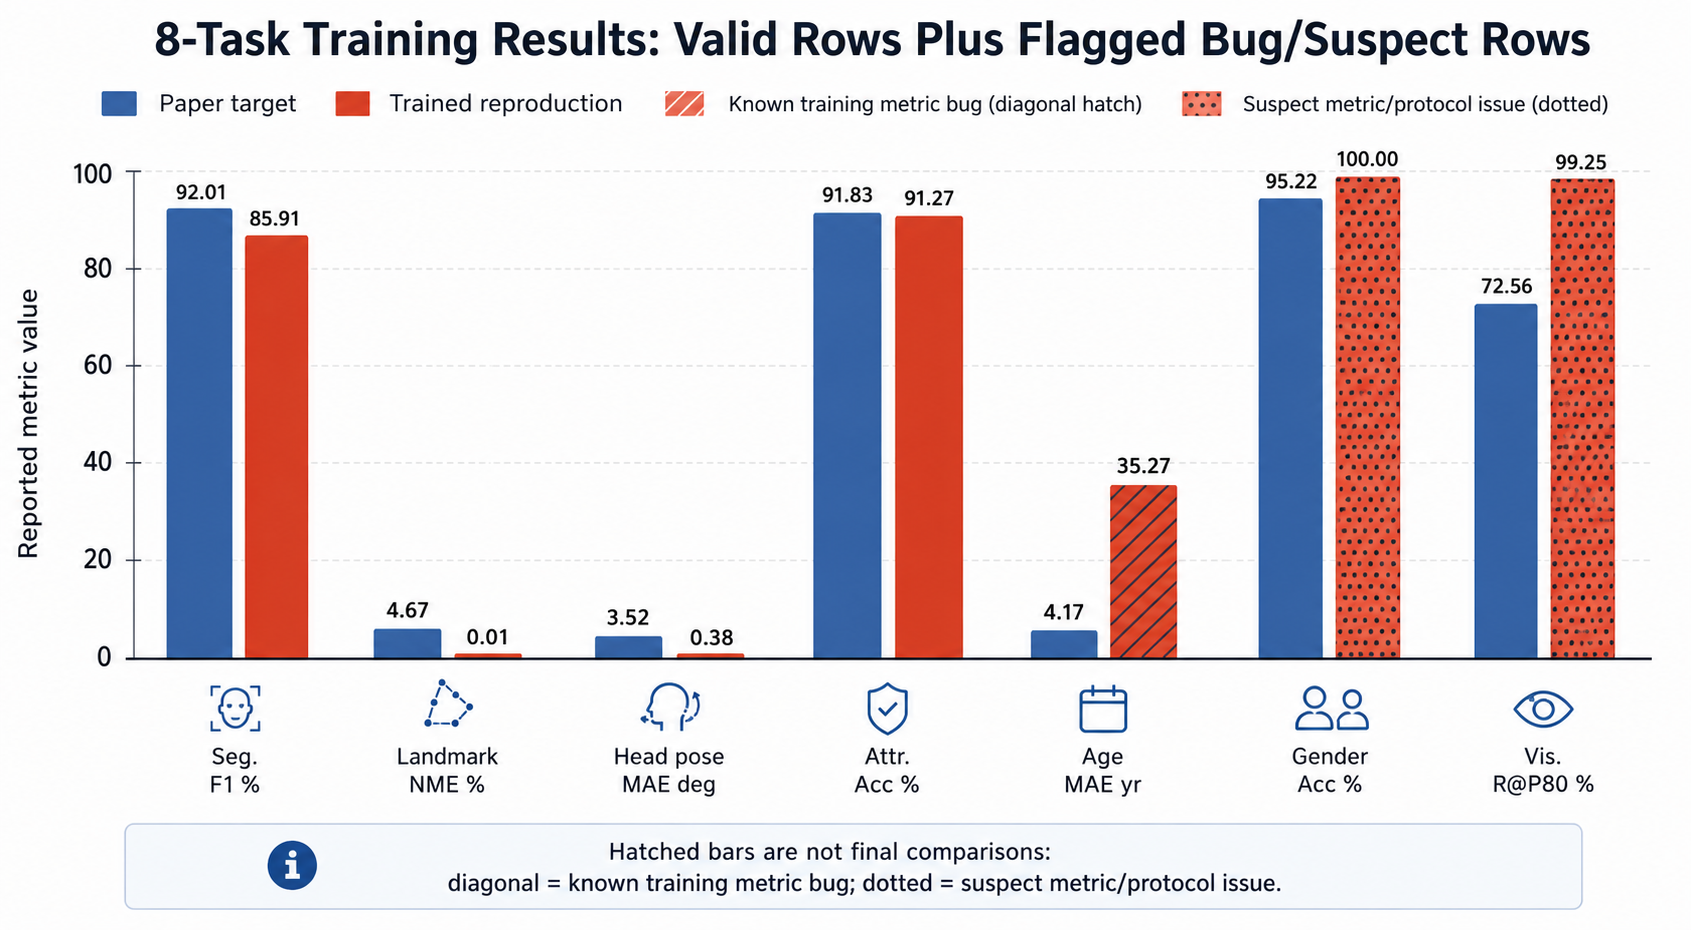
\includegraphics[width=0.98\textwidth]{assets/fig5_training_results_flagged.png}
\caption{Preliminary training results with bug-affected and suspect rows flagged.}
\end{figure}


\subsection{Analysis of Valid and Reportable Rows}


The segmentation result demonstrates that the rebuilt eight-task training pipeline is functional, but it does not match the paper. The trained model reaches 85.91\% F1 on CelebAMask-HQ compared with the paper target of 92.01\%, a gap of 6.10 percentage points. This gap is large enough to be meaningful. The most likely contributors are the architectural divergences documented in Section 3: the reproduced landmark task uses a single-token MLP head rather than the paper's 68-token hourglass design, which likely weakens the spatial gradient signal flowing into the shared representation. The missing expression and face recognition tasks may also reduce the diversity of co-training supervision. Finally, the paper mentions additional epochs for some tasks but does not specify which tasks receive them, so the uniform 12-epoch reproduction may undertrain segmentation relative to the original protocol.


Attribute prediction is the cleanest positive training result. CelebA attribute accuracy reaches 91.27\%, only 0.56 percentage points below the paper target of 91.83\%. This near-match supports the correctness of the CelebA loader, binary cross-entropy objective, task routing, and sampler behavior for at least one large classification task. It also aligns with the released-checkpoint baseline in Section 5, where CelebA attributes were one of the closest paper matches.


The UTKFace gender result of 85.04\% is plausible but does not have a direct paper target in the current table. FairFace gender at 100.00\% is not plausible as a clean scientific result and is therefore marked suspect. A saturated score can arise from class imbalance, label mapping errors, split issues, or an accuracy implementation that is not measuring the intended label set. FairFace race at 99.96\% is similarly suspect, especially because the current model head and FairFace source taxonomy do not align perfectly.


Visibility reaches 99.25\% Recall@P80 on COFW, far above the paper target of 72.56\%. This should not be interpreted as a strong improvement over the paper. Recall@P80 is sensitive to the exact precision-recall construction, label polarity, interpolation rule, and class balance in the visibility labels. A model or metric that predicts most landmarks as visible can appear strong under some recall-oriented summaries if the test split is dominated by visible landmarks. This row should be retained as a warning signal that the visibility protocol needs verification.


\subsection{Deferred Bug-Affected Analysis}


The detailed analysis of landmark, head pose, and age training failures is deferred until the bug-fixed retraining run is complete. The current values are useful only as evidence that the training evaluation path is faulty: landmark NME of 0.0117 is physically implausible, head-pose MAE of 0.379 is not safely interpretable without unit/protocol verification, and age MAE above 30 years indicates either a serious training failure, metric error, or both. These rows will be replaced and analyzed in the final report version after retraining.


\section{Discussion}


\subsection{What Worked: Validated Components}


Several components of the reproduction are validated by converging evidence across the released-checkpoint baseline and the trained eight-task run. The strongest signal is CelebA attribute prediction: the released checkpoint reaches 91.72\% against the paper target of 91.83\%, and the reproduced trained model reaches 91.27\%. These near-matches support the CelebA data loader, task routing, binary cross-entropy loss, metric normalization, and multi-task sampler for at least one large-scale classification task.


Segmentation provides a second, more qualified validation. The released checkpoint reaches 91.77\% F1, nearly matching the paper's 92.01\% target. The trained reproduction reaches 85.91\%, below the paper but still high enough to show that the rebuilt eight-task training pipeline is learning meaningful dense face representations rather than collapsing. The staged training strategy also worked operationally: it allowed the pipeline to be debugged first on geometric tasks, then expanded to classification tasks, and finally extended to the full eight-task reproduction scope.


\subsection{Failure Mode A: Metric Documentation Gaps}


The baseline evaluation exposed how easily a weights-only release can be misread when metric units are not documented with the same care as model architecture. Raw script outputs may be fractions, percentages, years, normalized coordinate errors, radians, or degrees. Without a normalization manifest, a valid result can look like a catastrophic failure, or a suspect result can look like a breakthrough. For example, a raw segmentation F1 fraction near 0.9177 corresponds to 91.77\%, which nearly matches the paper. Interpreting the raw fraction as a percentage would lead to an obviously wrong conclusion.


This is not merely a formatting problem. Metric normalization determines whether independent reproducers can compare results at all. The same checkpoint may appear to fail or succeed depending on whether the evaluator knows the unit convention, label mapping, and postprocessing rule. The fixed baseline manifest improves this by recording \path{raw_metric}, \path{normalized_metric}, \path{normalized_metric_unit}, and \path{normalization_rules}. A table like Table 4.5 should be considered part of the reproducibility artifact, not an optional reporting convenience.


\subsection{Failure Mode B: Multi-Task Loss Scale and Age}


The age rows are not final because the training evaluation bug affects them, but they still highlight a broader reproducibility risk: the paper's loss coefficients are underspecified. Multi-task training is not defined solely by the list of losses. It is defined by the relative scale at which those losses enter the optimizer. A Dice loss is bounded near the [0, 1] range, binary cross-entropy for a balanced binary decision is on the order of log(2), and a continuous age error can naturally live on a scale of tens of years if it is not normalized. Setting all task weights to 1.0 may therefore produce very different gradient magnitudes across tasks.


The reported preliminary age MAE above 30 years cannot yet be treated as a final result, but it is consistent with the kind of instability that loss-scale imbalance can create. The important reproducibility point does not depend on the final rerun value: lambda values are first-order hyperparameters in a multi-task system. Omitting them from the paper, appendix, and public code means that an independent reproducer must either guess, tune, or contact the authors. Future versions of this reproduction should test gradient-norm balancing, uncertainty weighting, or explicit loss normalization as controlled variants rather than treating \path{lambda_i = 1.0} as a harmless default.


\begin{figure}[H]
\centering
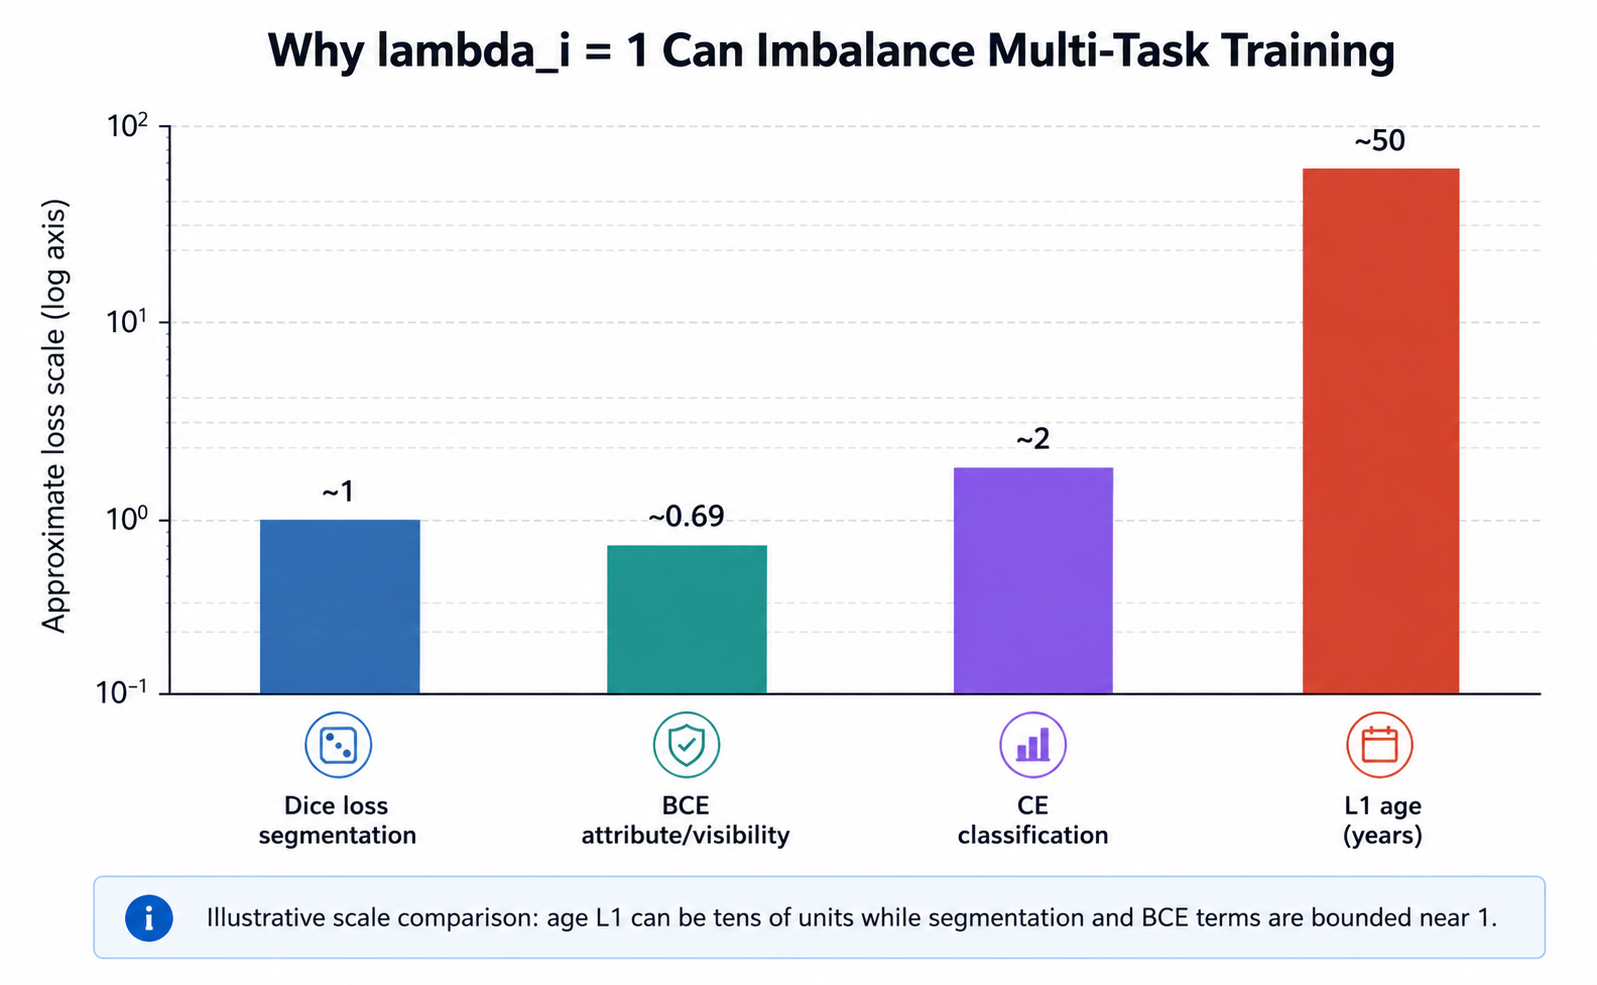
\includegraphics[width=0.78\textwidth]{assets/fig7_loss_scale_comparison.png}
\caption{Loss scale comparison across tasks.}
\end{figure}


\subsection{Failure Mode C: Architectural Divergence in Landmark and Head Pose}


The most consequential architectural divergence is the landmark pathway. The paper describes 68 landmark tokens and an hourglass landmark head. The reproduced implementation uses one landmark token followed by an MLP that emits all 136 coordinate values. This changes the role of landmark supervision in the shared representation. With 68 tokens, each keypoint can form its own query into the face representation and send localized gradients back through the FaceX decoder. With one token, that geometric signal is compressed before prediction, reducing the opportunity for per-keypoint attention and task-specific spatial feedback.


This may partly explain the segmentation gap in the trained model. Segmentation depends on high-quality spatial face tokens. If the landmark task provides weaker spatial supervision than the paper's architecture intended, the shared representation may be less precise, even if the segmentation head itself is implemented correctly. Head pose contains a related representation mismatch: the paper describes 9 rotation-matrix tokens, while the implementation predicts 3 Euler-angle values from one token. These divergences do not make the reproduction invalid, but they mean the reproduced model is not an exact implementation of the paper's architecture.


\subsection{What Remains To Be Done}


\begin{itemize}[leftmargin=*]
\item Fix the training/evaluation bug affecting landmark, head pose, and age, then rerun and report final values.
\item Verify BIWI head-pose preprocessing, axis convention, crop generation, and rotation conversion against the original protocol.
\item Verify COFW Recall@P80 against the paper definition, including label polarity, thresholding, and interpolation.
\item Investigate FairFace gender/race saturated or near-saturated values by checking split composition, label mapping, and class distributions.
\item Run a controlled loss-weighting study, including \path{lambda_i = 1.0}, tuned weights, and gradient-norm balancing.
\item Extend the reproduction to the full ten-task setting if resources permit: expression recognition with RAF-DB/AffectNet and face recognition with MS1MV3 plus PartialFC/ArcFace.
\end{itemize}

\subsection{Implications for Reproducibility Standards}


The main lesson is that the unit of reproducibility is the complete training pipeline, not the pretrained checkpoint. A checkpoint can verify that some inference behavior is real, as the segmentation and attribute baselines show. It cannot explain how the model was trained, how datasets were sampled, how losses were weighted, how augmentations were applied, or how ambiguous metrics were normalized. For a multi-task model, those choices are not secondary. They define the experiment.


Metric documentation should be treated as infrastructure. Papers and repositories should publish the raw metric convention, normalized reporting unit, label mapping, and evaluation protocol for every task. This is especially important when a single model spans segmentation, regression, classification, verification, and precision-recall metrics. Without this documentation, independent evaluation becomes a guessing exercise even when the checkpoint loads successfully.


Loss coefficients also need to be reported explicitly. In a single-task model, a missing scalar may be harmless; in a multi-task model, the lambda vector determines how tasks compete for shared representation capacity. Requiring private email confirmation for these values is not sufficient for scientific reproducibility. A reproducible release should include training code, dataset adapters or exact preprocessing instructions, sampler logic, loss definitions, loss coefficients, evaluation scripts, metric normalization rules, and checkpoint metadata.


\section{Conclusion}


This project reconstructed the FaceXFormer training and evaluation pipeline for eight of the ten tasks claimed in the original paper. We rebuilt dataset loaders, task-specific preprocessing, augmentation logic, multi-task sampling, loss functions, distributed training, checkpointing, and metric normalization. The final reproduction scope covers segmentation, landmark detection, head pose estimation, attribute prediction, age estimation, gender classification, race classification, and visibility prediction, trained through a staged 3-to-6-to-8 task schedule on 8 x A100 hardware.


The released checkpoint is broadly credible for some core tasks: segmentation and CelebA attribute prediction match the paper within one percentage point after proper metric normalization. The trained eight-task reproduction also produces meaningful segmentation and a close CelebA attribute result, showing that the reconstructed pipeline is functional. However, landmark, head pose, and age remain under active repair because of identified training/evaluation bugs, and several demographic or visibility rows require protocol verification before they can be interpreted as final scientific results.


The main contribution of this work is therefore not just a set of reproduced numbers. It is a concrete documentation of what a weights-only release does and does not make reproducible. FaceXFormer's architecture appears sound, but independent reproduction required reconstructing the training system, resolving paper-vs-code divergences, obtaining missing loss-weight information, and building a metric normalization framework. For multi-task models, reproducibility must include the complete training pipeline, not only the checkpoint.


\appendix
\section{Repository and Checkpoint Details}

\emph{Table A.1. Reproducibility Metadata}

\begingroup
\scriptsize
\setlength{\tabcolsep}{3pt}
\begin{longtable}{@{}>{\RaggedRight\arraybackslash}p{0.380\textwidth}>{\RaggedRight\arraybackslash}p{0.380\textwidth}@{}}
\toprule
Field & Value \\
\midrule
\endfirsthead
\toprule
Field & Value \\
\midrule
\endhead
Baseline scope & Current eight-task implementation \\
Tasks & Segmentation, landmark, headpose, attribute, age, gender, race, visibility \\
Checkpoint file & \path{checkpoints/ckpts/model.pt} \\
Checkpoint SHA256 & \texttt{327A755849BA64D3\allowbreak{}36FB96589FF87B27\allowbreak{}E84A12BE1ECF8BCF\allowbreak{}AA503D66F803286D} \\
Checkpoint size & 1,104,869,851 bytes \\
Checkpoint loadable & Yes (\path{checkpoint_loaded: true}) \\
Baseline evaluation generated & 2026-04-28T11:38:36 \\
Dataset root & \path{D:\Projects\facexformer-main\datasets\datasets} \\
Batch size & 64 \\
Seed & 0 \\
Number of result rows & 14 \\
Total evaluated samples & 129,060 \\
Result CSV & \path{results/baseline_current_8task_fresh_fixed/gap_analysis_baseline_current_8task.csv} \\
Result JSON & \path{results/baseline_current_8task_fresh_fixed/gap_analysis_baseline_current_8task.json} \\
Manifest & \path{results/baseline_current_8task_fresh_fixed/baseline_current_8task_manifest.json} \\
Repository & \path{https://github.com/kamrul28890/FaceXFormer-a-unified-transformer} \\
\bottomrule
\end{longtable}
\endgroup


\emph{Normalization rules from manifest.}

\begingroup
\scriptsize
\setlength{\tabcolsep}{3pt}
\begin{longtable}{@{}>{\RaggedRight\arraybackslash}p{0.380\textwidth}>{\RaggedRight\arraybackslash}p{0.380\textwidth}@{}}
\toprule
Task group & Rule \\
\midrule
\endfirsthead
\toprule
Task group & Rule \\
\midrule
\endhead
Segmentation & Raw F1 fraction multiplied by 100 gives percent \\
Attribute / Gender / Race & Raw accuracy fraction multiplied by 100 gives percent \\
Visibility & Raw recall fraction multiplied by 100 gives percent \\
Head pose & Raw MAE is already degrees in the fixed manifest \\
Landmark & Raw NME is already percent; normalized-coordinate datasets use sqrt(2) as image diagonal \\
Age & Raw MAE is already years; bucket targets are converted to representative age-bin centers \\
\bottomrule
\end{longtable}
\endgroup


\section{Raw Baseline Metrics}

\emph{Table B.1. Full Raw vs. Normalized Baseline Metrics}

\begingroup
\scriptsize
\setlength{\tabcolsep}{3pt}
\begin{longtable}{@{}>{\RaggedRight\arraybackslash}p{0.117\textwidth}>{\RaggedRight\arraybackslash}p{0.117\textwidth}>{\RaggedRight\arraybackslash}p{0.117\textwidth}>{\RaggedRight\arraybackslash}p{0.117\textwidth}>{\RaggedRight\arraybackslash}p{0.117\textwidth}>{\RaggedRight\arraybackslash}p{0.117\textwidth}>{\RaggedRight\arraybackslash}p{0.117\textwidth}>{\RaggedRight\arraybackslash}p{0.117\textwidth}@{}}
\toprule
Task & Dataset & Samples & Raw Metric & Normalized Metric & Unit & Paper Target & Normalized Gap \\
\midrule
\endfirsthead
\toprule
Task & Dataset & Samples & Raw Metric & Normalized Metric & Unit & Paper Target & Normalized Gap \\
\midrule
\endhead
Segmentation & CelebAMaskHQ & 2,000 & 0.9177 & 91.77 & percent & 92.01 & -0.24 \\
Landmark & 300W full & 689 & 6.7528 & 6.75 & NME percent & 4.67 & +2.08 \\
Landmark & 300W common & 554 & 5.5955 & 5.60 & NME percent & - & - \\
Landmark & 300W challenging & 135 & 11.5021 & 11.50 & NME percent & - & - \\
Head Pose & BIWI & 15,678 & 20.6497 & 20.65 & degrees & 3.52 & +17.13 \\
Attribute & CelebA & 19,962 & 0.9172 & 91.72 & percent & 91.83 & -0.11 \\
Attribute & LFWA & 13,143 & 0.6106 & 61.06 & percent & - & - \\
Age & UTKFace & 3,556 & 1.1714 & 1.17 & years & 4.17 & -3.00 \\
Age & FairFace & 21,908 & 6.2990 & 6.30 & years & - & - \\
Gender & UTKFace & 3,556 & 0.9918 & 99.18 & percent & - & - \\
Gender & FairFace & 21,908 & 0.9311 & 93.11 & percent & - & - \\
Race & UTKFace & 3,556 & 0.9803 & 98.03 & percent & - & - \\
Race & FairFace & 21,908 & 0.6459 & 64.59 & percent & - & - \\
Visibility & COFW & 507 & 0.8713 & 87.13 & percent & 72.56 & +14.57 \\
\bottomrule
\end{longtable}
\endgroup


\emph{Source: \path{results/baseline_current_8task_fresh_fixed/gap_analysis_baseline_current_8task.json}.}

\section{Figure List}

\begingroup
\scriptsize
\setlength{\tabcolsep}{3pt}
\begin{longtable}{@{}>{\RaggedRight\arraybackslash}p{0.280\textwidth}>{\RaggedRight\arraybackslash}p{0.280\textwidth}>{\RaggedRight\arraybackslash}p{0.280\textwidth}@{}}
\toprule
Figure & Title & Source / Generation \\
\midrule
\endfirsthead
\toprule
Figure & Title & Source / Generation \\
\midrule
\endhead
Fig. 3.1 & FaceXFormer end-to-end pipeline & \path{assets/fig1_facexformer_pipeline.png}; redrawn from paper architecture description \\
Fig. 3.2 & FaceX decoder block detail & \path{assets/fig2_facex_decoder_block.png}; drawn from TSA, TFCA, FTCA decoder description \\
Fig. 4.1 & Gap analysis summary heatmap & \path{assets/fig8_gap_analysis_heatmap.png}; generated from Table 4.1 impact labels \\
Fig. 4.2 & Staged training strategy timeline & \path{assets/fig3_staged_training_timeline.png}; generated from staged 3-to-6-to-8 task schedule \\
Fig. 5.1 & Baseline inference results bar chart & \path{assets/fig4_baseline_inference_bars.png}; generated from fixed baseline JSON \\
Fig. 6.1 & Preliminary training results with flagged rows & \path{assets/fig5_training_results_flagged.png}; generated from report instruction/final presentation values \\
Fig. 7.1 & Loss scale comparison across tasks & \path{assets/fig7_loss_scale_comparison.png}; illustrative loss-scale comparison \\
\bottomrule
\end{longtable}
\endgroup


The final presentation's embedded architecture image was also extracted for reference at \path{assets/pptx_media/image1.png}.


\section{Supplementary Implementation Notes}

\begin{enumerate}[leftmargin=*]
\item \textbf{STARLoss implementation.} The reproduced landmark loss is STARLoss-style and is applied to the MLP output coordinates. This differs from the paper's described 68-token hourglass landmark head.

\item \textbf{Head pose representation.} The paper describes 9 tokens representing a 3x3 rotation matrix. The reproduced implementation predicts three Euler-angle values from one pose token and converts them to rotation matrices for geodesic-loss computation where needed.

\item \textbf{Segmentation class mapping.} The paper states that segmentation uses one token per class, and the appendix mentions 19 CelebAMask-HQ classes. The reproduced implementation uses 11 segmentation/mask tokens. This is treated as a class-mapping ambiguity and architectural divergence.

\item \textbf{Age bins.} The reproduced implementation uses eight age bins with representative age-bin centers. This differs from the outline's earlier 11-bin assumption and should be treated as an implementation decision where the paper is underspecified.

\item \textbf{FairFace race mapping.} FairFace provides seven race categories, while the reproduced model head uses a five-class race output. FairFace race evaluation is therefore diagnostic rather than directly paper-comparable.

\item \textbf{COFW Recall@P80.} Visibility evaluation is sensitive to label polarity, class balance, precision-recall interpolation, and threshold selection. The COFW row is marked suspect until the exact paper protocol is verified.

\item \textbf{Loss coefficients.} The reported paper-faithful reproduction uses \path{lambda_i = 1.0} for all reproduced tasks based on author email confirmation. The paper and public release do not document these coefficients.

\item \textbf{Training results provenance.} The preliminary training metrics in Section 6 are taken from the report instruction/final presentation source. The raw bug-fixed training screenshot or log file was not present in the current repository package, so those rows are documented as provenance-tagged preliminary results rather than final bug-fixed training metrics.
\end{enumerate}

\end{document}
